% Plantilla realizada por Alberto Brunete (UPM). Basada en la de Santiago Morante Cendrero (UC3M)

%parametros de tipo libro
\documentclass[10pt,a4paper]{book}

%idioma español y acentos
\usepackage[spanish, es-tabla]{babel}
%\usepackage[latin1]{inputenc}
\usepackage[utf8]{inputenc}

%algunos símbolos matemáticos y paquete para usar subimágenes
\usepackage{amsmath}
\usepackage{amsfonts}
\usepackage{amssymb}
\usepackage{graphicx}
\usepackage{subfigure}
\usepackage{listings}
\usepackage[title,titletoc,toc]{appendix}
%Márgenes
\usepackage[left=3cm,top=3cm,right=3cm,bottom=3cm]{geometry}
\usepackage{url}

\usepackage{pdflscape}
\usepackage{changepage}
%
\usepackage{multicol}

\usepackage{longtable}

\usepackage{float}
\usepackage{eurosym}
\usepackage[usenames]{color}

 \definecolor{pRojo}{RGB}{255,30,30}
 \definecolor{pAmarillo}{RGB}{255,203,15}
 \definecolor{pAzul}{RGB}{60,145,188}
 \definecolor{pVerde}{RGB}{92,196,123}
 \definecolor{pGris}{RGB}{69,69,69}

 %para generar índice con hipervínculos
 \usepackage{hyperref}


\usepackage[xindy,toc,acronyms,nonumberlist]{glossaries}
 %\usepackage[xindy,acronym,toc,nonumberlist,sort=use]{glossaries} % nomain, if you define glossaries in a file, and you use \include{INP-00-glossary}
 \makeglossaries
 \usepackage[xindy]{imakeidx}
 \makeindex

 \loadglsentries[main]{capitulos/glosario}
% or using \input:
%\input{INP-00-glossary}

\graphicspath{figuras/} %path de los gráficos

%parametros del documento (sus propiedades)
\hypersetup{
    pdftitle={Nombre del alumno - TFG - año},
    pdfsubject={TFG - año},
    pdfauthor={Nombre del alumno},
    pdfkeywords={palabraclave1} {palabraclave2} {palabraclave3},
    colorlinks,
    citecolor=black,
    filecolor=black,
    linkcolor=black,
    urlcolor=black,
}


% %%%%%%%%% SUPER COMANDOS %%%%%%%%%%
\newcommand{\completar}{\textcolor{pRojo}{\small{\textbf{-- COMPLETAR --}}}}
\newcommand{\completarCon}[1]{ \textcolor{pRojo}{\small{\MakeUppercase{\textbf{#1}}}}}
\newcommand{\ingles}[1]{\textit{#1}}
\newcommand{\glosario}[1]{\ingles{\gls{#1}}}
\newcommand{\glosarioPlural}[1]{\ingles{\glspl{#1}}}
\newcommand{\minititulo}[1]{\subsection{#1}}
%\newcommand{\minititulo}[1]{{\vspace{\baselineskip}
%                            {\Large\textbf{#1}}
%                            \vspace{0.5\baselineskip plus 0pt}
%                            \normalsize}
%                            }
\newcommand{\codigo}[1]{\ttfamily{#1}\normalfont}
\newcommand{\iconoImagen}[1]{\centering \includegraphics[width=0.25\textwidth]{figuras/Imagenes_Piezas/#1.PNG}}
%width height
% %%%%%%%%%%%%%%%%%%%%%%%%%%%%%%%%%%%


%empieza el documento
\begin{document}

% %elementos antes del trabajo en sí se meten dentro de frontmatter
 \frontmatter

% %cada incluye referencia a un archivo de tipo .tex
 \begin{titlepage}
\begin{center}

%forma de introducir imágenes. el \\[0.5 cm] de final de línea introduce un salto de ese tamaño.
%width=1\textwidth indica el tamaño de la imágen (valores entre 0-1). 
 
\includegraphics[width=1\textwidth]{figuras/cabecera.png}  \\[0.5 cm]

\LARGE UNIVERSIDAD POLITÉCNICA DE MADRID \\ [1 cm]

\LARGE ESCUELA TÉCNICA SUPERIOR DE INGENIERÍA Y DISEÑO INDUSTRIAL \\ [1 cm]

\LARGE Grado en Ingeniería Electrónica y Automática Industrial\\ [1 cm]

\LARGE \textbf{TRABAJO FIN DE GRADO}\\[1 cm]

\Huge \textsc{Título del trabajo}\\[1 cm]

\LARGE Autor \\[2 cm]

%flushleft alinea a la izquierda el texto

\begin{multicols}{2} 
\begin{flushleft} \Large
\emph{Cotutor (si lo hay):} nombre y apellidos \\
\emph{Departamento:} departamento
\end{flushleft}

\begin{flushleft} \Large
\emph{Tutor:} nombre y apellidos\\
\emph{Departamento:} departamento
\end{flushleft}

\end{multicols} 

%rellena de blanco el resto de la página para escribir abajo del todo
\vfill

% Bottom of the page
{\large Ciudad, Mes año}

\end{center}
\end{titlepage}

 \begin{titlepage}
\begin{center}

%forma de introducir imágenes. el \\[0.5 cm] de final de línea introduce un salto de ese tamaño.
%width=1\textwidth indica el tamaño de la imágen (valores entre 0-1). 
 
\includegraphics[width=1\textwidth]{figuras/cabecera.png}  \\[0.5 cm]

\LARGE UNIVERSIDAD POLITÉCNICA DE MADRID \\ [1 cm]

\LARGE ESCUELA TÉCNICA SUPERIOR DE INGENIERÍA Y DISEñO INDUSTRIAL \\ [1 cm]

\LARGE Grado en Ingeniería Electrónica y Automática Industrial\\ [1 cm]

\LARGE \textbf{TRABAJO FIN DE GRADO}\\[1 cm]

\Huge \textsc{Diseño y construcción de un brazo robótico para el apoyo a la interactividad de personas enfermas}\\[3 cm]

\Large Firma Autor \\[2 cm]

%flushleft alinea a la izquierda el texto

\begin{multicols}{2} 
\begin{flushleft} 
\Large \emph{Firma Cotutor}
\end{flushleft}

\begin{flushright} 
\Large \emph{Firma Tutor}
\end{flushright}

\end{multicols} 

%rellena de blanco el resto de la página para escribir abajo del todo
\vfill

\end{center}
\end{titlepage}

 %Licencia opcional
 %\begin{flushleft}

Copyright \copyright  2018. Enrique Heredia Aguado

%ejemplo de licencia, se puede elegir cualquier otra

Esta obra está licenciada bajo la licencia Creative Commons Atribución-CompartirIgual 4.0 International (CC BY-SA 4.0). Para ver una copia del resumen de esta licencia, visite https://creativecommons.org/licenses/by-nd/4.0/. Puede acceder al código legal de la misma en https://creativecommons.org/licenses/by-nd/4.0/legalcode



\includegraphics[width=0.3\textwidth]{figuras/ccbysa.png}


Todas las opiniones aquí expresadas son del autor, y no reflejan necesariamente las opiniones
de la Universidad Politécnica de Madrid.

\end{flushleft}


 \cleardoublepage

\begin{flushleft} \large
\textbf{Título:} Diseño y construcción de un brazo robótico para el apoyo a la interactividad de personas enfermas \\
\textbf{Autor:} Henrique Heredia Aguado\\
\textbf{Tutor:} Miguel Hernando Gutiérrez \\ 
\textbf{Cotutor:} Alberto Brunete González\\ [1 cm]

\end{flushleft} 

\begin{center} \LARGE
EL TRIBUNAL \\ [1 cm]
\end{center}

\begin{flushleft} \LARGE
Presidente: Miguel Hernando Gutiérrez \\ [1 cm]
Vocal: Alberto Brunete González \\ [1 cm]
Secretario: Cecilia García Cena \\ [1.5 cm]
\end{flushleft}

\large
Realizado el acto de defensa y lectura del Trabajo Fin de Grado el día 28 de Febrero de 2018 en Madrid, en la Escuela Técnica Superior de Ingeniería y Diseño Industrial de la Universidad Politécnica de Madrid, acuerda otorgarle la CALIFICACIÓN de: \\ [2 cm]

\begin{center}
 \large VOCAL \\ [2.2 cm]
\end{center}

\begin{minipage}{0.5\textwidth}
 \begin{flushleft}
 \large SECRETARIO
\end{flushleft}
\end{minipage}
\begin{minipage}{0.5\textwidth}
\begin{flushright}
 \large PRESIDENTE
\end{flushright} 
\end{minipage}

 \chapter{Agradecimientos} \label{chap:Agradecimientos}

Agradezco a ............

 %chapter introduce un nuevo capítulo
\chapter{Resumen}

Este proyecto se resume en.................

\paragraph{Palabras clave:} palabraclave1, palabraclave2, palabraclave3.

\chapter{Abstract}

In this project...

\paragraph{Keywords:} keyword1, keyword2, keyword3.

 %genera índice
 \tableofcontents

% %índice de figuras.
 \listoffigures

 %índice de tablas.
 \listoftables

 %\glsaddall
 %\printglossary[type={main,acronym}]
 %\printglossary[type=\acronymtype]
 \printglossaries 
% TODO: \glsaddall

 %empieza la parte descriptiva del trabajo
 \mainmatter

 \chapter{Introducción} \label{chap:Introduccion}
\chapterimage{figuras/ImagenesPortada/PortadaIntro.jpg}
\hrule
\vspace{3mm}

En este capítulo se perfila la estructura, organización y contenidos principales del documento así como la motivación y objetivos del proyecto.


\section{Motivación del proyecto}



\section{Objetivos}

El objetivo que este Trabajo de Fin de Grado persigue es el del diseño, construcción y control de brazo robótico previo estudio de las opciones comerciales disponibles y su posible adaptación. Este proyecto está enmarcado bajo el proyecto Robohealth, proyecto financiado por el Ministerio de Economía y Competitividad con el objetivo del diseño de sistemas robóticos y domóticos para entornos hospitalarios que mejoren el sistema de salud actual. (\completar http://robohealth.es/)
\\

El  prototipo debe estar diseñado para una completa adaptación a un entorno hospitalario en el que deberá estar en contacto constante con usuarios a los que deberá respetar.
\\

El objetivo del brazo robótico es el de ubicar ante un paciente una \ingles{tablet}. Ésta llevará montado un dispositivo de seguimiento de vista de forma que, a través del movimiento de las pupilas, el paciente podrá interactuar con el resto de dispositivos de la habitación así como el personal médico. Es necesario motorizar el dispositivo para mantener el dispositivo de seguimiento siempre a una distancia y ángulo, respecto a la cara del paciente, mínima para facilitar el funcionamiento del mismo. Está pensado principalmente para pacientes con movilidad reducida o sin movilidad (temporal o permanente), aunque también podría agilizar la interfaz humano-habitación para el resto de pacientes.
\\

Así pues, algunos aspectos claves del prototipo deben ser:
\begin{itemize}
    \item El Objetivo del prototipo será el de permitir una interacción más cómoda y automatizada entre los pacientes cuya capacidad de interacción se ha visto reducida por la causa que sea.
    \item Se debe tener en cuenta es que el prototipo estará en constante contacto con gran variedad de usuarios: pacientes, médicos, familiares, etc. El diseño debe proteger en todo momento la seguridad de dichos usuarios
    \item Concretamente el diseño está pensado para interactuar con pacientes que se encuentran recostados en una camilla en el hospital.
\end{itemize}

\subsection{Objetivos derivados}

La realización de dicho prototipo implica el cumplimiento de otros objetivos secundarios o derivados del principal. Se pueden listar algunos como:
\begin{itemize}
    \item Prueba de diferentes tipos de estructuras y materiales como base física del brazo robótico.
    \item Adquisición de conocimientos sobre modelado 3D digital así como diferentes métodos de fabricación como son la impresión 3D, el corte láser, fresado CNC así como el uso de otras herramientas de mecanizado más tradicionales.
    \item Diseño e implementación de un sistema de control en cascada, que permita un control en posición y en velocidad del brazo robótico.
    \item Trabajar con protocolos de comunicación serie a bajo nivel (Comunicación entre el robot y el exterior exterior además de la comunicación con los actuadores).
    \item Diseñar una interfaz que permita controlar el brazo de manera intuitiva (interfaz gráfica o similar).
\end{itemize}


\section{Estructura del documento}

El documento está organizado de tal forma que irá introduciendo al lector progresivamente en los diferentes aspectos del diseño y montaje del prototipo mencionado, desde aspectos más generales hasta los más técnicos.
\\

Los capítulos están a su vez organizados en el orden que se seguiría de cara a montar el prototipo empezando por una base física, añadiendo a posteriori los componentes electromecánicos para finalizar con los aspectos de control. Concretamente los capítulos contienen la siguiente información:

\begin{itemize}
    \item Como continuación de los requerimientos generales se encuentra descritos en la introducción, en el capítulo \ref{chap:estadoarte}, un estudio de diferentes modelos y diseños comerciales que podrían adaptarse para cumplir los objetivos presentados.
    \item El estudio del estado del arte ayuda a definir las ideas más importantes que regirán el diseño del prototipo. Éstas consideraciones se presentan en el capítulo \ref{chap:Punto_partida}.
    \item El capítulo \ref{chap:Mecanica} entra de lleno en los aspectos mecánicos del brazo robótico, pasando por una valoración de distintas posibilidades para llegar al diseño definitivo.
    \item Continuando con la descripción de soporte físico, el capítulo \ref{chap:Cinematica} supone un cambio de perspectiva que guiará al lector desde la parte mecánica y física expuesta anteriormente a la descripción matemática y cinemático del modelo.
    \item Una vez descrito el soporte físico del brazo robótico se detalla el hardware escogido para su puesta en marcha. En el capítulo \ref{chap:Electronica} presentan los componentes electromecánicos que se han integrado en prototipo; sus características principales así como su ubicación en el montaje.
    \item El análisis de la estructura software diseñado queda cubierto en el capítulo \ref{chap:SW}. Este apartado anticipa además algunas ideas sobre el sistema de control diseñado.
    \item Continuando con las pinceladas aportadas en el apartado anterior, el capítulo \ref{chap:Control} expone de forma detallada los distintos aspectos de diseño y desarrollo del control del brazo.
    \item Una vez alcanzado este punto, habiendo cubierto los aspectos del diseño del brazo, el capítulo \ref{chap:Resultados} recoge los resultados de funcionamiento de prototipo para ser analizados.
    \item No se dejan de lado aspectos de gestión, costes y viabilidad del prototipo que se detallan en el capítulo \ref{chap:Gestion}.
    \item Finalmente, el capítulo \ref{chap:Conclusiones} expone las conclusiones finales del trabajo así como posibles desarrollos futuros.
\end{itemize}

Como complemento a la información que exponen los apartados de esta memoria se añaden al final diferentes anexos:

\begin{itemize}
    \item Se adjunta un listado de todas las piezas diseñadas con información relevante sobre su uso y fabricación en el anexo \ref{app:listadoPiezas}.
    \item Vistas las piezas que conforman el prototipo es importante localizarlas para entender su uso y diseño. El anexo \ref{app:montajePiezas} detalla unas pautas y orden para el ensamblado del prototipo. Además permite localizar en su contexto las piezas listadas en el anexo \ref{app:listadoPiezas}.
    \item Volviendo sobre los aspectos del software, en el Anexo \ref{app:codificacionSW} se concretan las reglas de codificación, mencionadas en el capítulo \ref{chap:SW}, más relevantes que se han aplicado en el desarrollo del código.
    \item De igual forma se amplia la información sobre el software desarrollado en el anexo \ref{app:documentacion_software}. En él se encuentra la documentación del software generada a través de la herramienta \glosario{doxygen}.
    \item El desarrollo del proyecto conlleva la utilización de diferentes herramientas software cuya instalación y puesta apunto se detalla en el anexo \ref{app:instalacion_software}.
\end{itemize}

\section{Software utilizado}

Aunque en el anexo \ref{app:instalacion_software} se detalla la instalación del software en más detalle no está de más conocer las herramientas a utilizar de antemano, ya que éstas marcan unas pautas en la ideología de diseño y una estructura a la hora de ordenar y desarrollar el proyecto.

\begin{itemize}
    \item Autodesk Inventor 2016: Es un software de modelado paramétrico 3D de la compañía Autodesk Inc.
    \item Atom: Se trata de un editor de texto \ingles{open source}. Permite la instalación de diferentes extensiones para ampliar sus utilidades, entre otras será necesario instalar \glosario{PlatformIO}, que convierte el editor en un \glosario{IDE} completo para el desarrollo de software para diferentes placas como Arduino, que será la base de este proyecto.
    \item Matlab: herramienta de cálculo utilizada para analizar la información recogida del ámbito de control así como para las comprobaciones pertinentes sobre la cinemática.
    \item Lizard: Software que permite el análisis de la complejidad de código. Se compone de una serie de scripts en python que, al ser ejecutados devuelven un fichero con métricas de complejidad referentes a los ficheros de código sobre los que se invoca: complejidad ciclomática, número de funciones en cada fichero, líneas de código en cada función y fichero, entre otras..
    \item Cloc: Es una herramienta sencilla que cuenta, de forma más precisa, el número de líneas de código, comentarios y líneas en blanco de los ficheros de código.
    \item cpplint: Análisis del cumplimiento de las reglas de codificación en el software. Es una herramienta desarrollada en python por Google LLC para asegurar que los proyectos cumplen con sus reglas de codificación, que se han seguido de forma parcial en este proyecto. Se pueden ver los aspectos más relevantes de las reglas de codificación en el Anexo \ref{app:codificacionSW}.
    \item doxygen: Permite la generación de documentación para código de diferentes lenguajes, c++ en este caso, de forma automática. La herramienta obtiene comentarios del código, escritos con una sintaxis determinada, para documentar los diferentes métodos, objetos y estructura del software.
\end{itemize}


\section{Iconografía del proyecto}

Se han diseñado y utilizado diferentes iconos que pueden servir para orientar el propósito o temática de las diferentes figuras incluidas en el documento así como el capítulo al que pertenecen, manteniendo un color uniforme a lo largo de cada capítulo. Además de tener en la figura \ref{fig:introduccion:iconos} una recopilación de los mismos, a continuación se expone una lista con su significado y capítulo al que se asocia.
\begin{figure}[H]
	\centering
	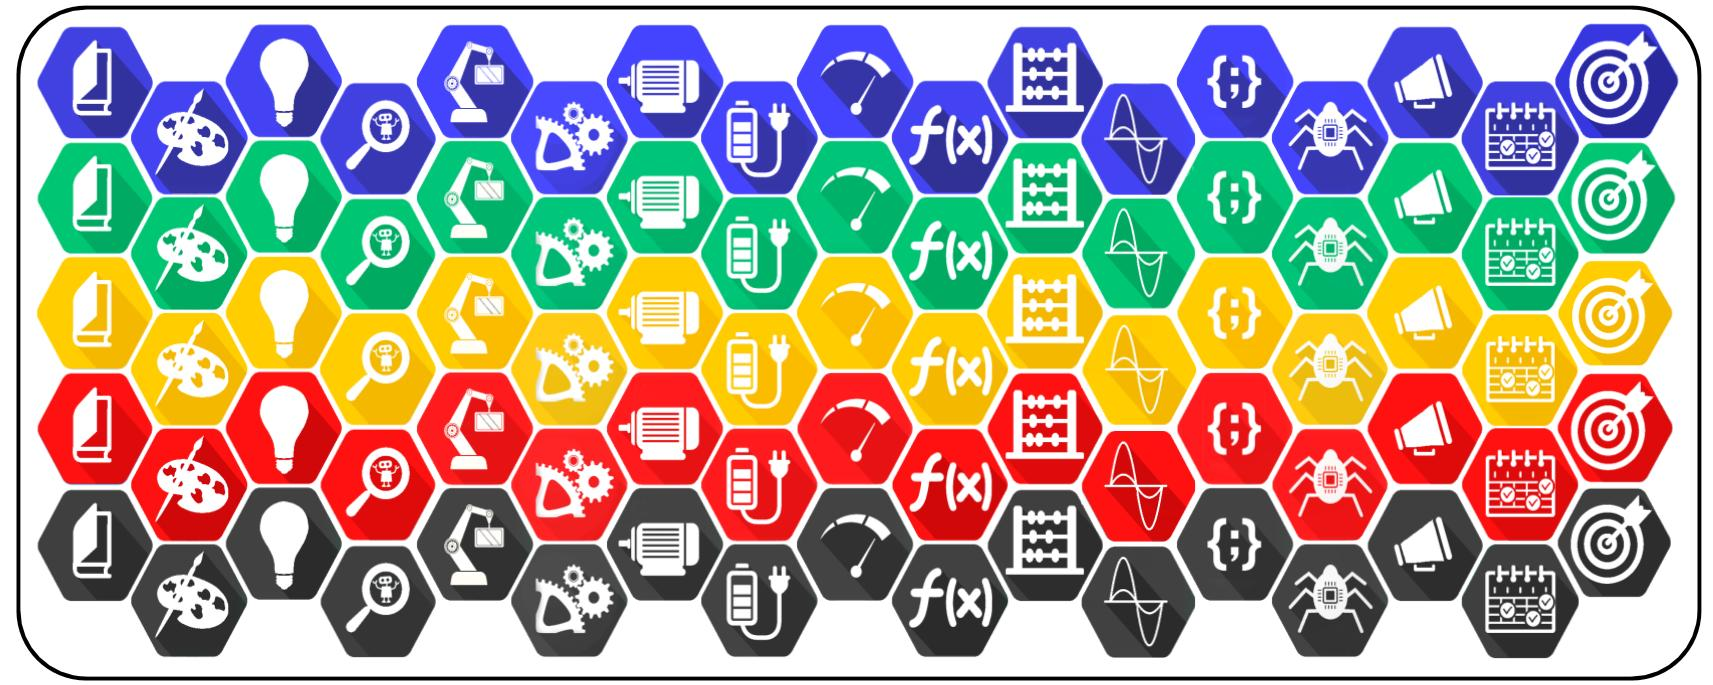
\includegraphics[width=\textwidth]{figuras/Icons/iconos.jpg}
	\caption{Recopilación de los iconos diseñados y utilizados}
	\label{fig:introduccion:iconos}
	\immagesource{Autor}
\end{figure}

\begin{multicols}{2} 
	\begin{flushleft} 
		\subsection*{Capítulo 1: Introducción}
		\inconExplanation{intro_yellow}{Introducción, apertura del proyecto}
	\end{flushleft}	
		
	\begin{flushright} 
		\subsection*{Capítulo 2: Estado del arte}
		\inconExplanation{arte_blue}{Aspectos relacionados con el estado del arte}
	\end{flushright}
\end{multicols} 

\subsection*{Capítulo 3: Punto de inicio del diseño}
\begin{multicols}{2} 
	\begin{flushleft} 
		\inconExplanation{lupa_yellow}{Detalles sobre el robot}
	\end{flushleft}	
	
	\begin{flushright} 
		\inconExplanation{idea_yellow}{Ideas de interés}
	\end{flushright}
\end{multicols} 

\subsection*{Capítulo 4: Mecánica}
\begin{multicols}{2} 
	\begin{flushleft} 
		\inconExplanation{brazo_red}{Aspectos generales de la estructura del brazo robótico}
	\end{flushleft}
	
	\begin{flushright} 
		\inconExplanation{mecanismo_red}{Transmisión mecánica de movimiento}
	\end{flushright}	
\end{multicols} 

\subsection*{Capítulo 5: Electromecánica}
\begin{multicols}{2} 
	\begin{flushleft} 
		\inconExplanation{motor_green}{Actuadores para el brazo robótico}
	\end{flushleft}
	
	\begin{flushright} 
		\inconExplanation{bateria_green}{Alimentación y etapas de potencia}
	\end{flushright}
\end{multicols} 
\begin{multicols}{2}
	\begin{flushleft} 
		\inconExplanation{velocidad_green}{Sensores para el brazo robótico}	
	\end{flushleft}
\end{multicols} 

\subsection*{Capítulo 6: Estudio matemático}
\begin{multicols}{2} 
	\begin{flushleft} 
		\inconExplanation{math_red}{Ecuaciones y relaciones matemáticas}
	\end{flushleft}
	
	\begin{flushright} 
		\inconExplanation{abaco_red}{Resultados calculados}
	\end{flushright}
\end{multicols} 

\begin{multicols}{2} 
	\begin{flushleft} 
		\subsection*{Capítulo 7: Aspectos de Control}
		\inconExplanation{control_yellow}{Gráficas y aspectos del control}
	\end{flushleft}
\end{multicols} 

\subsection*{Capítulo 8: Software}
\begin{multicols}{2} 
	\begin{flushleft} 
		\inconExplanation{llaves_blue}{Diseño y desarrollo del software}
	\end{flushleft}
	
	\begin{flushright} 
		\inconExplanation{debug_blue}{Test, verificación y debug del software desarrollado}
	\end{flushright}	
\end{multicols} 

\begin{multicols}{2} 
	\begin{flushleft} 
		\subsection*{Capítulo 9: Resultados y discusión}
		\inconExplanationOne{megafono_red}
	\end{flushleft}
	\begin{flushright} 
		\subsection*{Capítulo 10: Gestión del proyecto}
		\inconExplanation{agenda_green}{Gestión del proyecto}
	\end{flushright}
\end{multicols} 

\begin{multicols}{2} 
	\begin{flushleft} 
		\subsection*{Capítulo 11: Conclusiones}
		\inconExplanation{diana_blue}{Conclusiones}
	\end{flushleft}
\end{multicols} 


 %partes finales del trabajo: conclusiones, bibliografia y anexos

 \chapter{Estado del arte} \label{chap:estadoarte}
\chapterimage{figuras/ImagenesPortada/PortadaEArte.jpg}
\hrule
\vspace{3mm}

Una vez se han repasado los aspectos generales que se buscan para este proyecto conviene hacer un estudio de la situación actual de modelos comerciales o de investigación con los que se puedan encontrar sinergias 
\\

De esta manera este capítulo hace un repaso de diferentes soluciones destinadas al soporte y posicionamiento de monitores, ordenadores o tablets. Además se hace referencia también a modelos de brazos robóticos específicamente destinados a la asistencia en entornos de usuarios. Dentro de todas las soluciones comerciales se centrará el estudio en las que están específicamente pensadas para su instalación en entornos médicos siempre que sea posible.
\\

Según el apoyo así como los tipos de grados de libertad hay diferentes configuraciones posibles, en este capítulo se verán algunos modelos concretos de cada caso evaluando sus características, ventajas e inconvenientes de los mismos de forma que se pueda generalizar a modelos equivalentes. De igual manera se podrán encontrar modelos motorizados y modelos sin motorizar, clasificación por la que serán agrupados a continuación.
\\

\section{Soportes articulados sin motorizar}

Dentro del grupo de soportes articulados sin motorizar se pueden clasificar según el tipo de anclaje que tienen, ya se enganchen al techo, pared, suelo, etc.
\\

Dentro de cada tipo de anclaje los soportes comerciales disponibles son bastante parecidos por lo que se presentará un modelo concreto que encaje dentro de las dimensiones y capacidad de carga requeridas para la aplicación que se pretende explotar para sacar conclusiones generales sobre cada tipo de soporte.

\subsection{Anclaje a la pared: Cotytech MW-M13P}

Dentro de esta gama (Cotytech MW-M*) se pueden encontrar modelos para soportar diferentes cargas. Concretamente se ha elegido el modelo con menores prestaciones y que soporta menos carga por ser suficiente para la aplicación que se pretende dar. Otros modelos pueden incluir soporte para teclado, caja y cobertura para cables y enganche a pared, entre otros, suponiendo un incremento sobre el precio de este modelo. Obtenida de \cite{CotytechMWM13P:2018} tenemos información relevante que se resume a continuación:

\begin{minipage}{0.35\textwidth}
	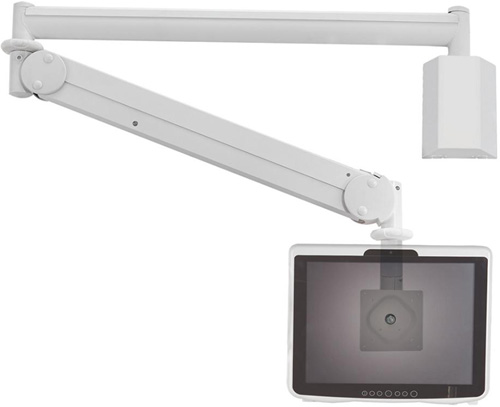
\includegraphics[width=\linewidth]{figuras/Imagenes_EstadoArte/Cotytech_MW-M13P.jpg}
\end{minipage}
\begin{minipage}{0.65\textwidth}\raggedright
	\hspace{1cm}
	\begin{itemize}
		\item Tipo de anclaje: Anclaje a la pared.
		\item Tipo de articulación: Articulaciones rotacionales.
		\item Capacidad de carga: entre $1kg$ y $6kg$.
		\item Extensión máxima: $185.7cm$.
		\item Número de grados de libertad: 5.
		\item Ángulos articulaciones: $370^o$ (brazo posición), $270^o$ (muñeca posición), $180^o$ (pared) $^1$. %fake footnote
		\item Ángulos de orientación: Tilt: $20^o$/- $35^o$ (muñeca orientación) y $20^o$/- $60^o$ (brazo orientación).
		\item Peso del soporte: $4.76 kg$.
		\item Precio estándar: 686.98\euro. $^2$. %fake footnote
	\end{itemize}
\end{minipage}

\begin{minipage}{1\textwidth}
	\footnotesize{$^1$En la imagen se pueden ver tres puntos articulados diferenciados, el punto que se fija a la pared con un grado de libertad, el punto central del brazo, que tiene dos grados de libertad (se separarán entre orientación y posición, aunque su efecto no está desacoplado)y la muñeca, que incluye la articulación que se aprecia justo encima de la pantalla como la rotacional sobre la que queda enganchada la misma (con una clasificación análoga al caso intermedio).}
	
    \footnotesize{$^2$Precio a pasado a Euros según el cambio oficial en el día consultado.}
\end{minipage}

 Paralelamente a este modelo la marca Cotytech tiene una versión que, manteniendo el mismo esquema de mecánico, permite un anclaje al techo: el modelo CM-M13 visto en \cite{CotytechCMM13:2018} con un coste de 853.06\euro.

\subsection{Anclaje al techo: Titan Elite T2EQ-C8X5}

 Concretamente se ha tomado el modelo con la montura doblada hacia arriba para un anclaje en el techo. La siguiente información constituye un resumen con los puntos más importantes vistos en \cite{TitanElite:2018}:

 \begin{minipage}{0.35\textwidth}
 	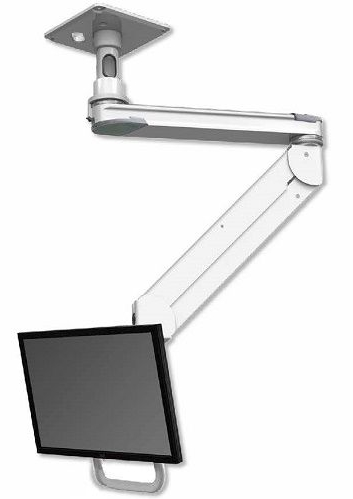
\includegraphics[width=\linewidth]{figuras/Imagenes_EstadoArte/T2EQ.jpg}
 \end{minipage}
 \begin{minipage}{0.65\textwidth}\raggedright
 	\hspace{1cm}
 	\begin{itemize}
 		\item Tipo de anclaje: Anclaje al techo.
 		\item Tipo de articulación: Articulaciones rotacionales.
 		\item Capacidad de carga: hasta $12.7kg$ en diferentes configuraciones.
 		\item Extensión máxima: $106cm$ (la longitud vertical del anclaje al techo variará según se elija al comprar).
 		\item Número de grados de libertad: 5.
 		\item Ángulos articulaciones: $360^o$ para las tres primeras articulaciones que rotan sobre el eje horizontal.
 		\item Ángulos de orientación: Tilt: $50^o$.
 		\item Peso del soporte: $9kg$.
 		\item Precio estándar: 628.30\euro.
 	\end{itemize}
 \end{minipage}
 \\

 Este mismo modelo cuenta con diferentes enganches y longitudes de los tubos que permiten anclarlo al suelo, al techo o a la pared indistintamente.

\subsection{Anclaje a una mesa o superficie de trabajo: Ergotron LX Sit-Stand Desk Arm}

 De entre la gama incluida en los modelos de Ergotron LX se ha elegido aquel que tenía unas dimensiones más ajustadas a las necesidades reales. En general el resto de la gama y otros soportes similares tienen unas dimensiones más reducidas. Resumidas de \cite{LXSitStand:2018} y \cite{LXSitStandWeb:2018} se encuentran a continuación las principales características del modelo:

 \begin{minipage}{0.35\textwidth}
 	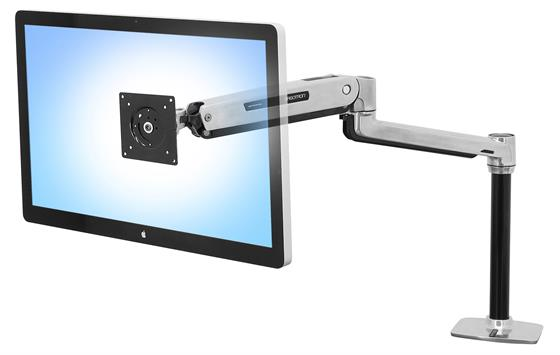
\includegraphics[width=\linewidth]{figuras/Imagenes_EstadoArte/LX_Sit-Stand_Desk_Arm.jpg}
 	\\

 	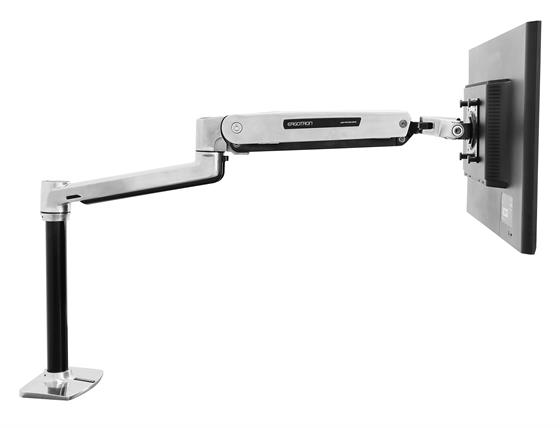
\includegraphics[width=\linewidth]{figuras/Imagenes_EstadoArte/LX_Sit-Stand_Desk_Arm_2.jpg}
 \end{minipage}
 \begin{minipage}{0.65\textwidth}\raggedright
 	\hspace{1cm}
 	\begin{itemize}
 		\item Tipo de anclaje: Anclaje a una mesa, camilla o similar.
 		\item Tipo de articulación: Primera articulación prismática, resto rotacionales.
 		\item Capacidad de carga: hasta $11.3kg$.
 		\item Extensión máxima: se puede variar hasta $36cm$ en altura (articulación prismática, esta es susceptible de ser modificada para ajustarla a otras alturas) y alcanza una extensión de $84cm$
 		\item Número de grados de libertad: 6 (una prismática y cinco rotacionales).
 		\item Ángulos articulaciones: $180^o$ la primera articulación, fija al anclaje; $360^o$ a mitad del brazo y $180^o$ en la muñeca.
 		\item Ángulos de orientación: Tilt: (giro sobre el eje medio horizontal de la pantalla) $75^o$; Pan (eje perpendicular a la pantalla): $360^o$.
 		\item Peso del soporte: $8.9kg$.
 		\item Precio estándar: 247.00\euro – 299.00\euro dependiendo de la tienda y configuración.
 	\end{itemize}
 \end{minipage}
 \\

 \vspace{0.1cm}
 Este mismo modelo cuenta con diferentes enganches y longitudes de los tubos que permiten anclarlo al suelo, al techo o a la pared indistintamente.

 \subsection{Consideraciones generales sobre los soportes no motorizados}
 Los modelos vistos hasta ahora presentan un rango de movimientos muy amplio, están certificados y preparados para su uso en entornos hospitalarios además de estar destinados precisamente al soporte de monitores. En todos los casos la capacidad de carga excede con creces la que se estima necesaria en este proyecto por lo que todas las opciones podrían ser válidas.
 \\

 Aunque cuentan con puntos bastante favorables se trata de productos cerrados sobre los cuales sería complicado integrar actuadores y sensores de manera adecuada, segura y en última instancia, elegante. Además el rango de precios en el que se encuentran es bastante elevado.

\section{Soportes articulados motorizados}

Se centrará este apartado en los modelos que se pueden ver en \cite{maiormover:2018}, como por ejemplo el MaiorFlip 900.

\begin{minipage}{0.35\textwidth}
   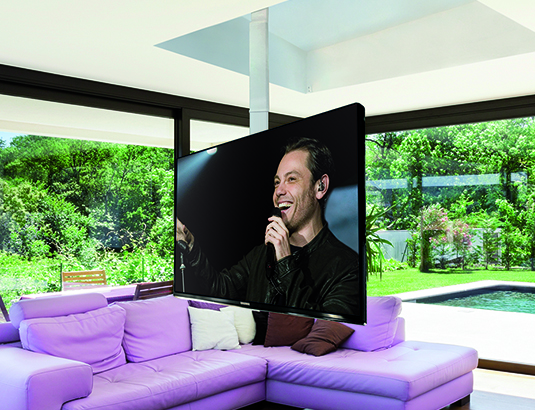
\includegraphics[width=\linewidth]{figuras/Imagenes_EstadoArte/not_valid_1.jpg}
\end{minipage}
\begin{minipage}{0.65\textwidth}\raggedright
   \hspace{1cm}
   \begin{itemize}
       \item Tipo de anclaje: Anclaje al techo.
       \item Tipo de articulación: Primera articulación rotacional, segunda prismática y tercera rotacional.
       \item Capacidad de carga: máximo de $28kg$.
       \item Extensión máxima: Descenso de hasta $68cm$
       \item Número de grados de libertad: 3 (una prismática y dos rotacionales).
       \item Ángulos articulaciones: Primera rotación giro de hasta $90^o$; articulación prismática con un alcance de $68cm$ con una capacidad de giro de la articulación final de $360^o$.
       \item Peso del soporte: $35kg$.
       \item Precio estándar: Bajo demanda.
   \end{itemize}
\end{minipage}
\\

 \vspace{0.1cm}
Otros modelos que se pueden encontrar presentan unas características similares:

\begin{minipage}{0.5\textwidth}
   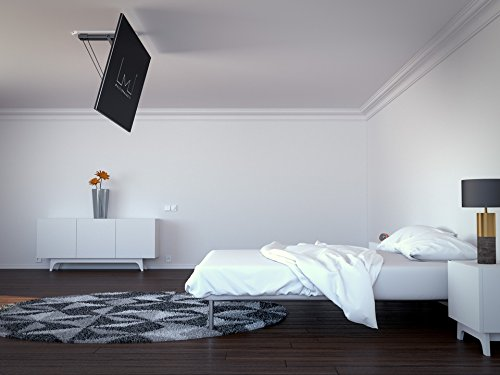
\includegraphics[width=0.8\linewidth]{figuras/Imagenes_EstadoArte/not_valid_2.jpg}
\end{minipage}
\begin{minipage}{0.5\textwidth}
   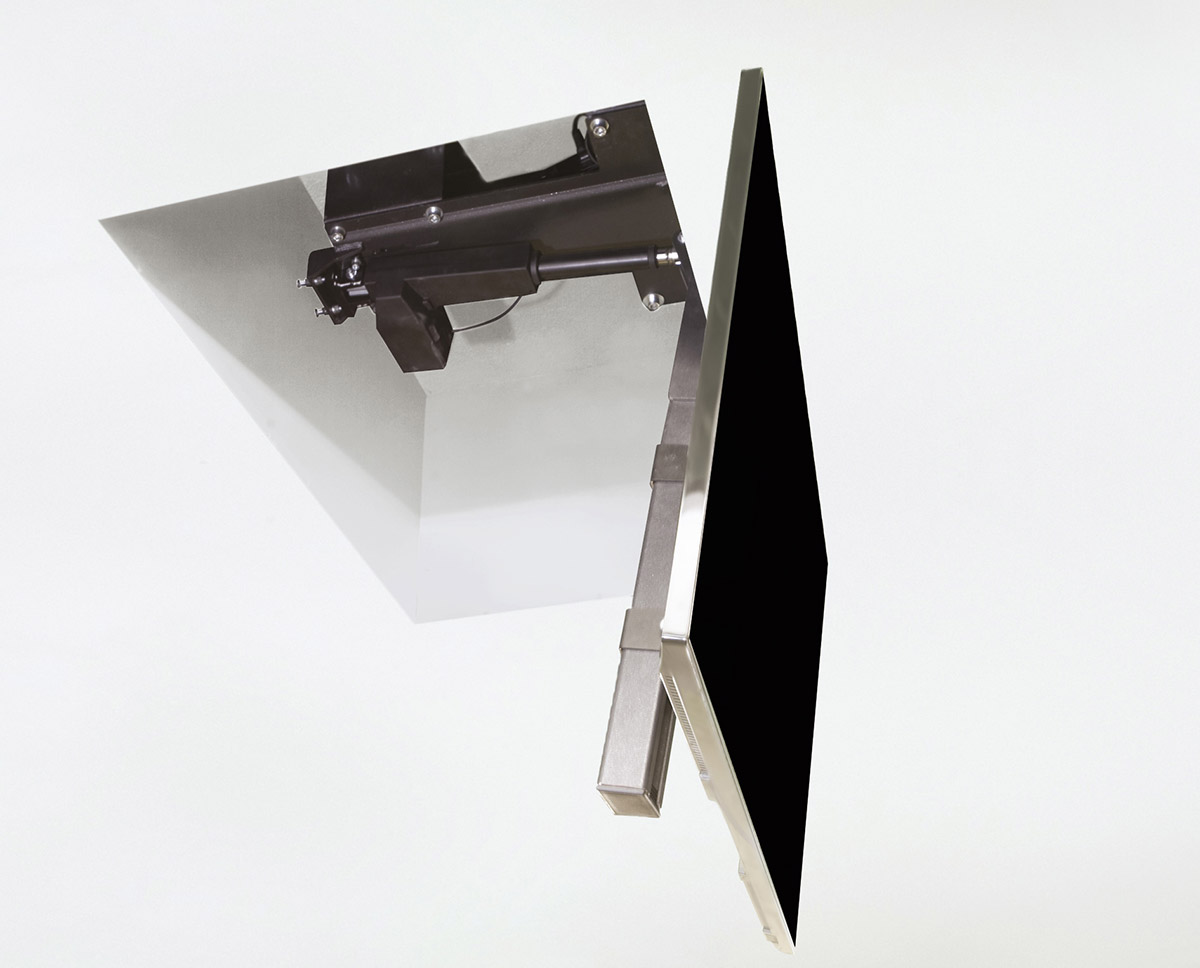
\includegraphics[width=0.8\linewidth]{figuras/Imagenes_EstadoArte/not_valid_3.jpg}
\end{minipage}
 \subsection{Consideraciones generales sobre los soportes motorizados}

    En esta línea podemos encontrar también los diseños de \cite{Chung2009} o \cite{ChungL.Chang2008}. Se puede ver también el modelo \cite{Chung2009} dotado de articulaciones paralelas que permiten controlar la orientación del dispositivo.
    \\
    
    Este tipo de soportes están principalmente pensados para motorizar televisores de gran tamaño con unos rangos de movimiento bastante limitados. Comúnmente presentan grados de libertad para modificar la orientación de la pantalla y en pocos casos un grado de libertad extra para desplazar, sobre algún eje el dispositivo.  No son aptos para la aplicación que se pretende dar puesto que no permiten su posicionamiento a una distancia adecuada del usuario.

\section{Brazos robóticos para asistencia de pacientes}

	En general para el propósito que se plantea en este proyecto se podría adaptar una solución robótica comercial implementando una interfaz entre la tablet y el controlador del brazo. En esta sección se presentan algunos modelos de brazos robóticos especialmente pensados como robots asistenciales, preparados para una interacción directa con pacientes en entornos hospitalarios o en casa.

 \subsection{JACO 3 fingers, Kinova robotics}
	 Pertenece a la línea de productos de Kinova robotics especialmente diseñados como robots asistenciales. Están pensados para una interacción directa con el paciente o usuario de forma que pueda convertirse en una extensión del mismo proporcionándole una mayor independencia. Entre las características descritas en \cite{Jaco:2018} y \cite{JacoWeb:2018} podemos recoger las siguientes más relevantes:
     \\

	  \begin{minipage}{0.35\textwidth}
	  	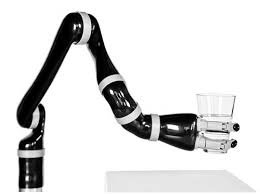
\includegraphics[width=\linewidth]{figuras/Imagenes_EstadoArte/jaco-3-finger.jpg}
	  \end{minipage}
	  \begin{minipage}{0.65\textwidth}\raggedright
	  	\hspace{1cm}
	  	\begin{itemize}
	  		\item Tipo de anclaje: Adaptativo a una mesa, silla de ruedas, etc
	  		\item Tipo de articulación: 6 grados de libertad rotacionales
	  		\item Capacidad de carga: entre $1.8kg$ y $1.6kg$ dependiendo de la versión elegida (con tres dedos tiene una capacidad menor).
	  		\item Extensión máxima: alcanza $90cm$.
	  		\item Número de grados de libertad: 6.
	  		\item Ángulos de posición: Rotación continua en las articulaciones.
	  		\item Ángulos de orientación: $55^o$ en la muñeca.
	  		\item Peso del brazo: $5.7kg$.
	  		\item Precio estándar: desde 34900\euro.
	  	\end{itemize}
	  \end{minipage}
	  \\

	  \vspace{0.1cm}

      Este modelo concreto, Jaco, viene en dos formatos pudiendo tener dos o tres dedos en el manipulador de su extremo.
      \\

	  De esta marca se puede adquirir también el modelo MICO con algo menos de alcance ($70cm$) como se ve en \cite{Mico:2018}. Los grados de libertad ofertados varían entre 4 y 7, se ha optado por tomar una solución lo más parecida a la requerida.

 \subsection{Brazo Multi-manipulador de la Universidad de Pamplona}

    Dejando de lado el ámbito puramente comercial se encuentran proyectos que es interesante repasar. En \cite{Marquez:2013} se describe un modelo diseñado específicamente como robot asistencial con capacidad de cambiar, de forma autónoma, entre diferentes manipuladores disponibles como pueden ser una cuchara, un tenedor, un cuenco, entre otros.
    \\

     \begin{minipage}{0.35\textwidth}
       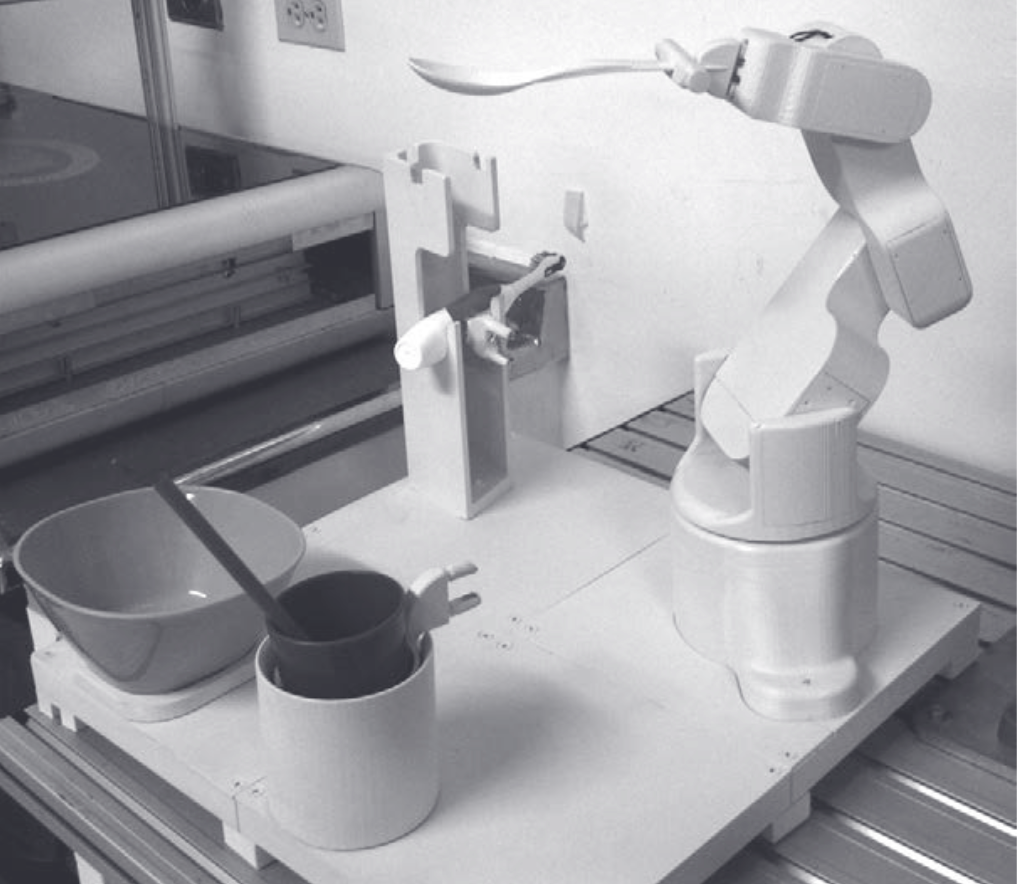
\includegraphics[width=\linewidth]{figuras/Imagenes_EstadoArte/UPamplona.png}
     \end{minipage}
     \begin{minipage}{0.65\textwidth}\raggedright
       \hspace{1cm}
       \begin{itemize}
           \item Tipo de anclaje: Lleva su propia plataforma sobre la que se monta
           \item Tipo de articulación: 4 grados de libertad rotacionales
           \item Capacidad de carga: manipuladores que adjunta.
           \item Extensión máxima: alcanza Superficie de trabajo de 40cm x 40cm.
           \item Número de grados de libertad: 4.
           \item Actuadores: Dynamixel AX-12
           \item Precio estándar: proyecto no comercial.
       \end{itemize}
     \end{minipage}
     \\

     \vspace{0.1cm}

     Es interesante destacar que aunque no se aportan demasiados datos sobre el modelo (peso del modelo, capacidad de giro de sus articulaciones, etc) si presenta un estudio completo de su aceptación así como facilidad de uso. Un sistema intuitivo es más fácilmente aceptado por los usuarios, a los cuales les será más fácil empezar a hacer uso de las facilidades que ofrece un robot de este tipo.
     \\

     Los actuadores que utiliza son de la gama de Dynamixel, una serie de servo motores muy versátiles aunque sin demasiada carga útil una vez montados sobre las articulaciones.

 \subsection{Brazo robótico para personas con movilidad reducida}

    Continuando con modelos de un ámbito más académico se encuentra el modelo descrito en \cite{Hideyuki:2010}. Se trata de un modelo plegable que puede ser almacenado o transportado dentro de una maleta de forma sencilla. Viene con un manipulador en forma de manopla que permite agarres de una amplia gama de objetos. También pensado para la asistencia de personas con movilidad reducida ha sido principalmente testeado para administrar alimentos y bebidas.
    \\

     \begin{minipage}{0.35\textwidth}
       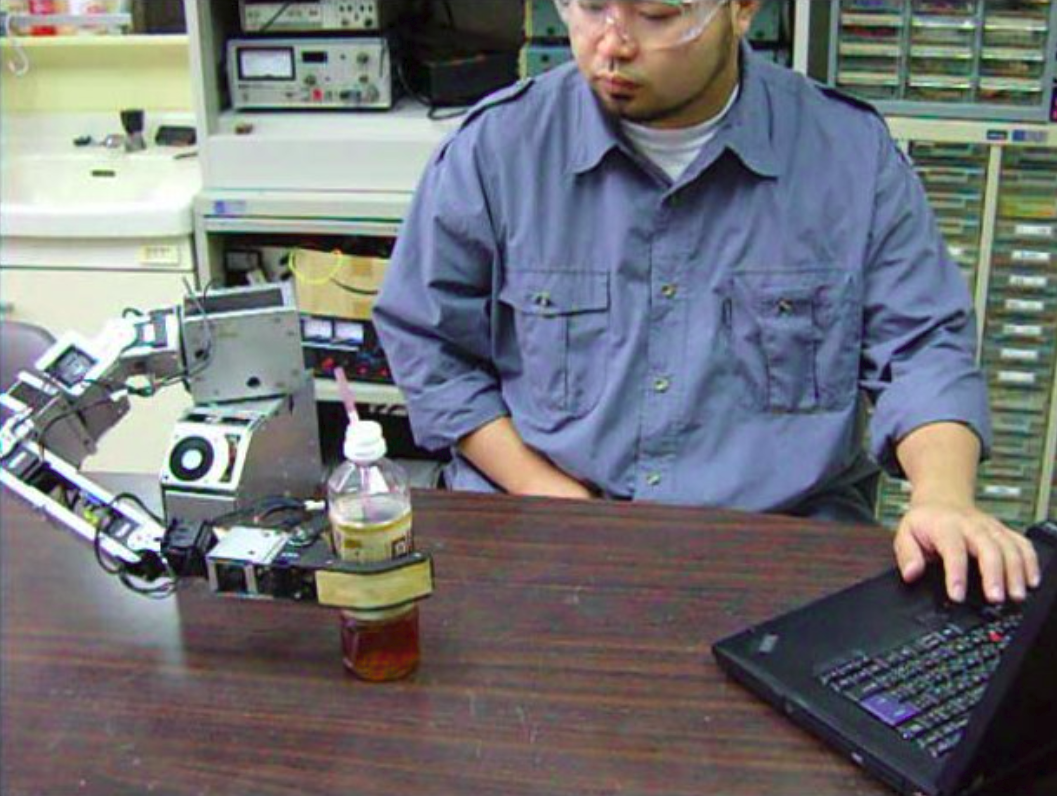
\includegraphics[width=\linewidth]{figuras/Imagenes_EstadoArte/Tokyo.png}
     \end{minipage}
     \begin{minipage}{0.65\textwidth}\raggedright
       \hspace{1cm}
       \begin{itemize}
           \item Tipo de anclaje: Sin determinar.
           \item Tipo de articulación: 7 grados de libertad rotacionales
   	  		\item Extensión máxima: alcanza $71cm$.
   	  		\item Número de grados de libertad: 7.
   	  		\item Peso del brazo: $5kg$ con dos baterías.
   	  		\item Precio estándar: proyecto no comercial.
       \end{itemize}
     \end{minipage}
     \\

     \vspace{0.1cm}
 \subsection{Consideraciones generales sobre los brazos robóticos}
 
	Además de los mencionados, en esta misma línea podemos encontrar otros modelos como \cite{Arai2011}, para ayuda a la alimentación, en \cite{Chang2003} diseñado específicamente para personas con movilidad reducida o \cite{Ali2007} presentando un prototipo asistencial genérico.
	\\
	
	Dentro de este formato conviene repasar el estudio hecho por \cite{Groothuis2013} en el cual se comparan diferentes modelos de brazos robóticos asistenciales en parámetros como movilidad, capacidad de carga y también seguridad.
	\\
	
    Aunque entre los modelos descritos sería fácil encontrar uno válido para la aplicación que se pretende dar, la mayoría de modelos comerciales (en los casos académicos se desconoce el precio que rondaría en caso de convertirse en producto comercial) tienen unos precios elevados que dificultarían su aplicación a gran escala.
    \\



 \chapter{Mecánica y soporte físico del proyecto} \label{chap:Mecanica}
\hrule
\vspace{3mm}

\section{Visión general} \label{sec:Mecanica:vision_general}

\section{Articulación uno. Giro en el eje Z} \label{sec:Mecanica:articulacion_uno}
    Junto con las articulaciones dos y tres, descritas en la Sección \ref{sec:Mecanica:articulacion_dostres} están consideradas como los grados de libertad que gestionan la posición del extremo del robot en un espacio tridimensional. En adelante se las podrá denominar también "grados de libertad de posición".
    
    Esta articulación está actuada por un \ingles{Servo G15 Cube} (descrito en la Sección \ref{sec:Introduccion:materiales_software}. El movimiento de dicho servo se transmite a la articulación a través de un juego de ruedas que, solidarias a la parte superior (parte móvil) de la articulación y por rozamiento, transmiten el movimiento hasta la pista inferior (parte fija a la base del robot).
    
    De esta forma aseguramos que el usuario, en cualquier momento podrá desplazar el robot superando el rozamiento de esta cadena de transmisión anulando, en caso de estar en proceso, el movimiento que pueda estar efectuando el \glosario{servo}.

\section{Articulaciones dos y tres. Posicionamiento en el plano sagital} \label{sec:Mecanica:articulacion_dostres}
    Estas dos articulaciones son las encargadas de posicionar el extremo en el plano sagital del robot.
    
    Están formadas por dos mecanismos de cuatro barras acoplados en serie. Tienen la particularidad de que las barras son iguales dos a dos, de forma que las barras se mantienen siempre en paralelo. Esta particularidad asegura que el extremo se mantenga siempre perpendicular al plano del suelo, de forma que se desacopla la orientación del extremo de la posición del mismo.
    
    \begin{figure}[H]
    \centering
    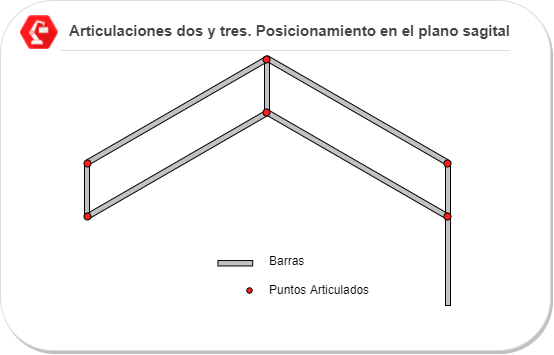
\includegraphics[width=0.75\textwidth]{figuras/mecanismos_4_barras.png}   
    \caption{Esquema de la cadena cinemática correspondiente a los \completarCon{Glosario a GDL} dos y tres}
    \label{fig:Mecanica:4_bar_mecanism}
    \end{figure}

\section{Posicionamiento de sensores y actuadores} \label{sec:Mecanica:sensores_actuadore}

\section{Estudio de la cadena cinemática completa} \label{sec:Mecanica:cadena_cinematica}

 \chapter{Diseño Electromecánico} \label{chap:Electronica}
\chapterimage{figuras/ImagenesPortada/PortadaElectronica.jpg}
\hrule
\vspace{3mm}

Aunque se han anticipado tanto textualmente como a través de imágenes algunas características de los componentes electrónicos utilizados aún no se han descrito en detalle. Este capítulo se mete de lleno en los aspectos electromecánicos del brazo robótico, haciendo una descripción de los componentes empleados, algunas pautas para su correcto uso así como su integración dentro de la estructura descrita en el capítulo \ref{chap:Mecanica}

\section{Actuadores} \label{sec:Electronica:Actuadores}
\label{sec:Electronica:Actuadores:G15}

    La imposición de utilizar unos motores de par reducido puede interpretarse como una desventaja, pero en este caso al quedar descartados los motores de corriente contínua y motores paso a paso convencionales queda la alternativa de uso de \glosarioPlural{smartservo} con todas las ventajas que ofrecen.
    \\

    Los \glosarioPlural{smartservo} elegidos para el proyecto son, concretamente, losG15 Cube de la marca Cytron. Estos servos vienen acompañados de una gran variedad de funcionalidades que facilitarán el control y manejo del brazo robótico. Estos servos, como la mayoría de \glosarioPlural{smartservo}, tienen implementado un sistema de comunicación bidireccional con la placa controladora a través de un tipo de comunicación conocida como \ingles{Half Serial Duplex Communication}. Como se cuenta en \cite{embeddedSystems}, este tipo de comunicación utiliza un solo cable que podrá operar en una u otra dirección cada vez. Puede darse la situación en que varios componentes intenten comunicar al mismo tiempo en ambas direcciones pudiendo ocasionar graves problemas en la electrónica de los mismos. El uso de este tipo de servos implica el uso de electrónica adicional, no solo a modo de etapa de potencia, si no para la gestión de la comunicación entre los mismos y el microcontrolador.
    \\

    Utilizar un protocolo de comunicación más complejo permite conectar varios servos a un mismo puerto de comunicación, conectando cada servo al anterior, también conocido como conexión \ingles{daisy chain}. En la figura \ref{fig:Electronica:bus-servos} se puede ver representada este tipo de cadena y donde se puede ver el aspecto del modelo de servos seleccionado.
    \\
    
    \begin{figure}[H]
    	\centering
    	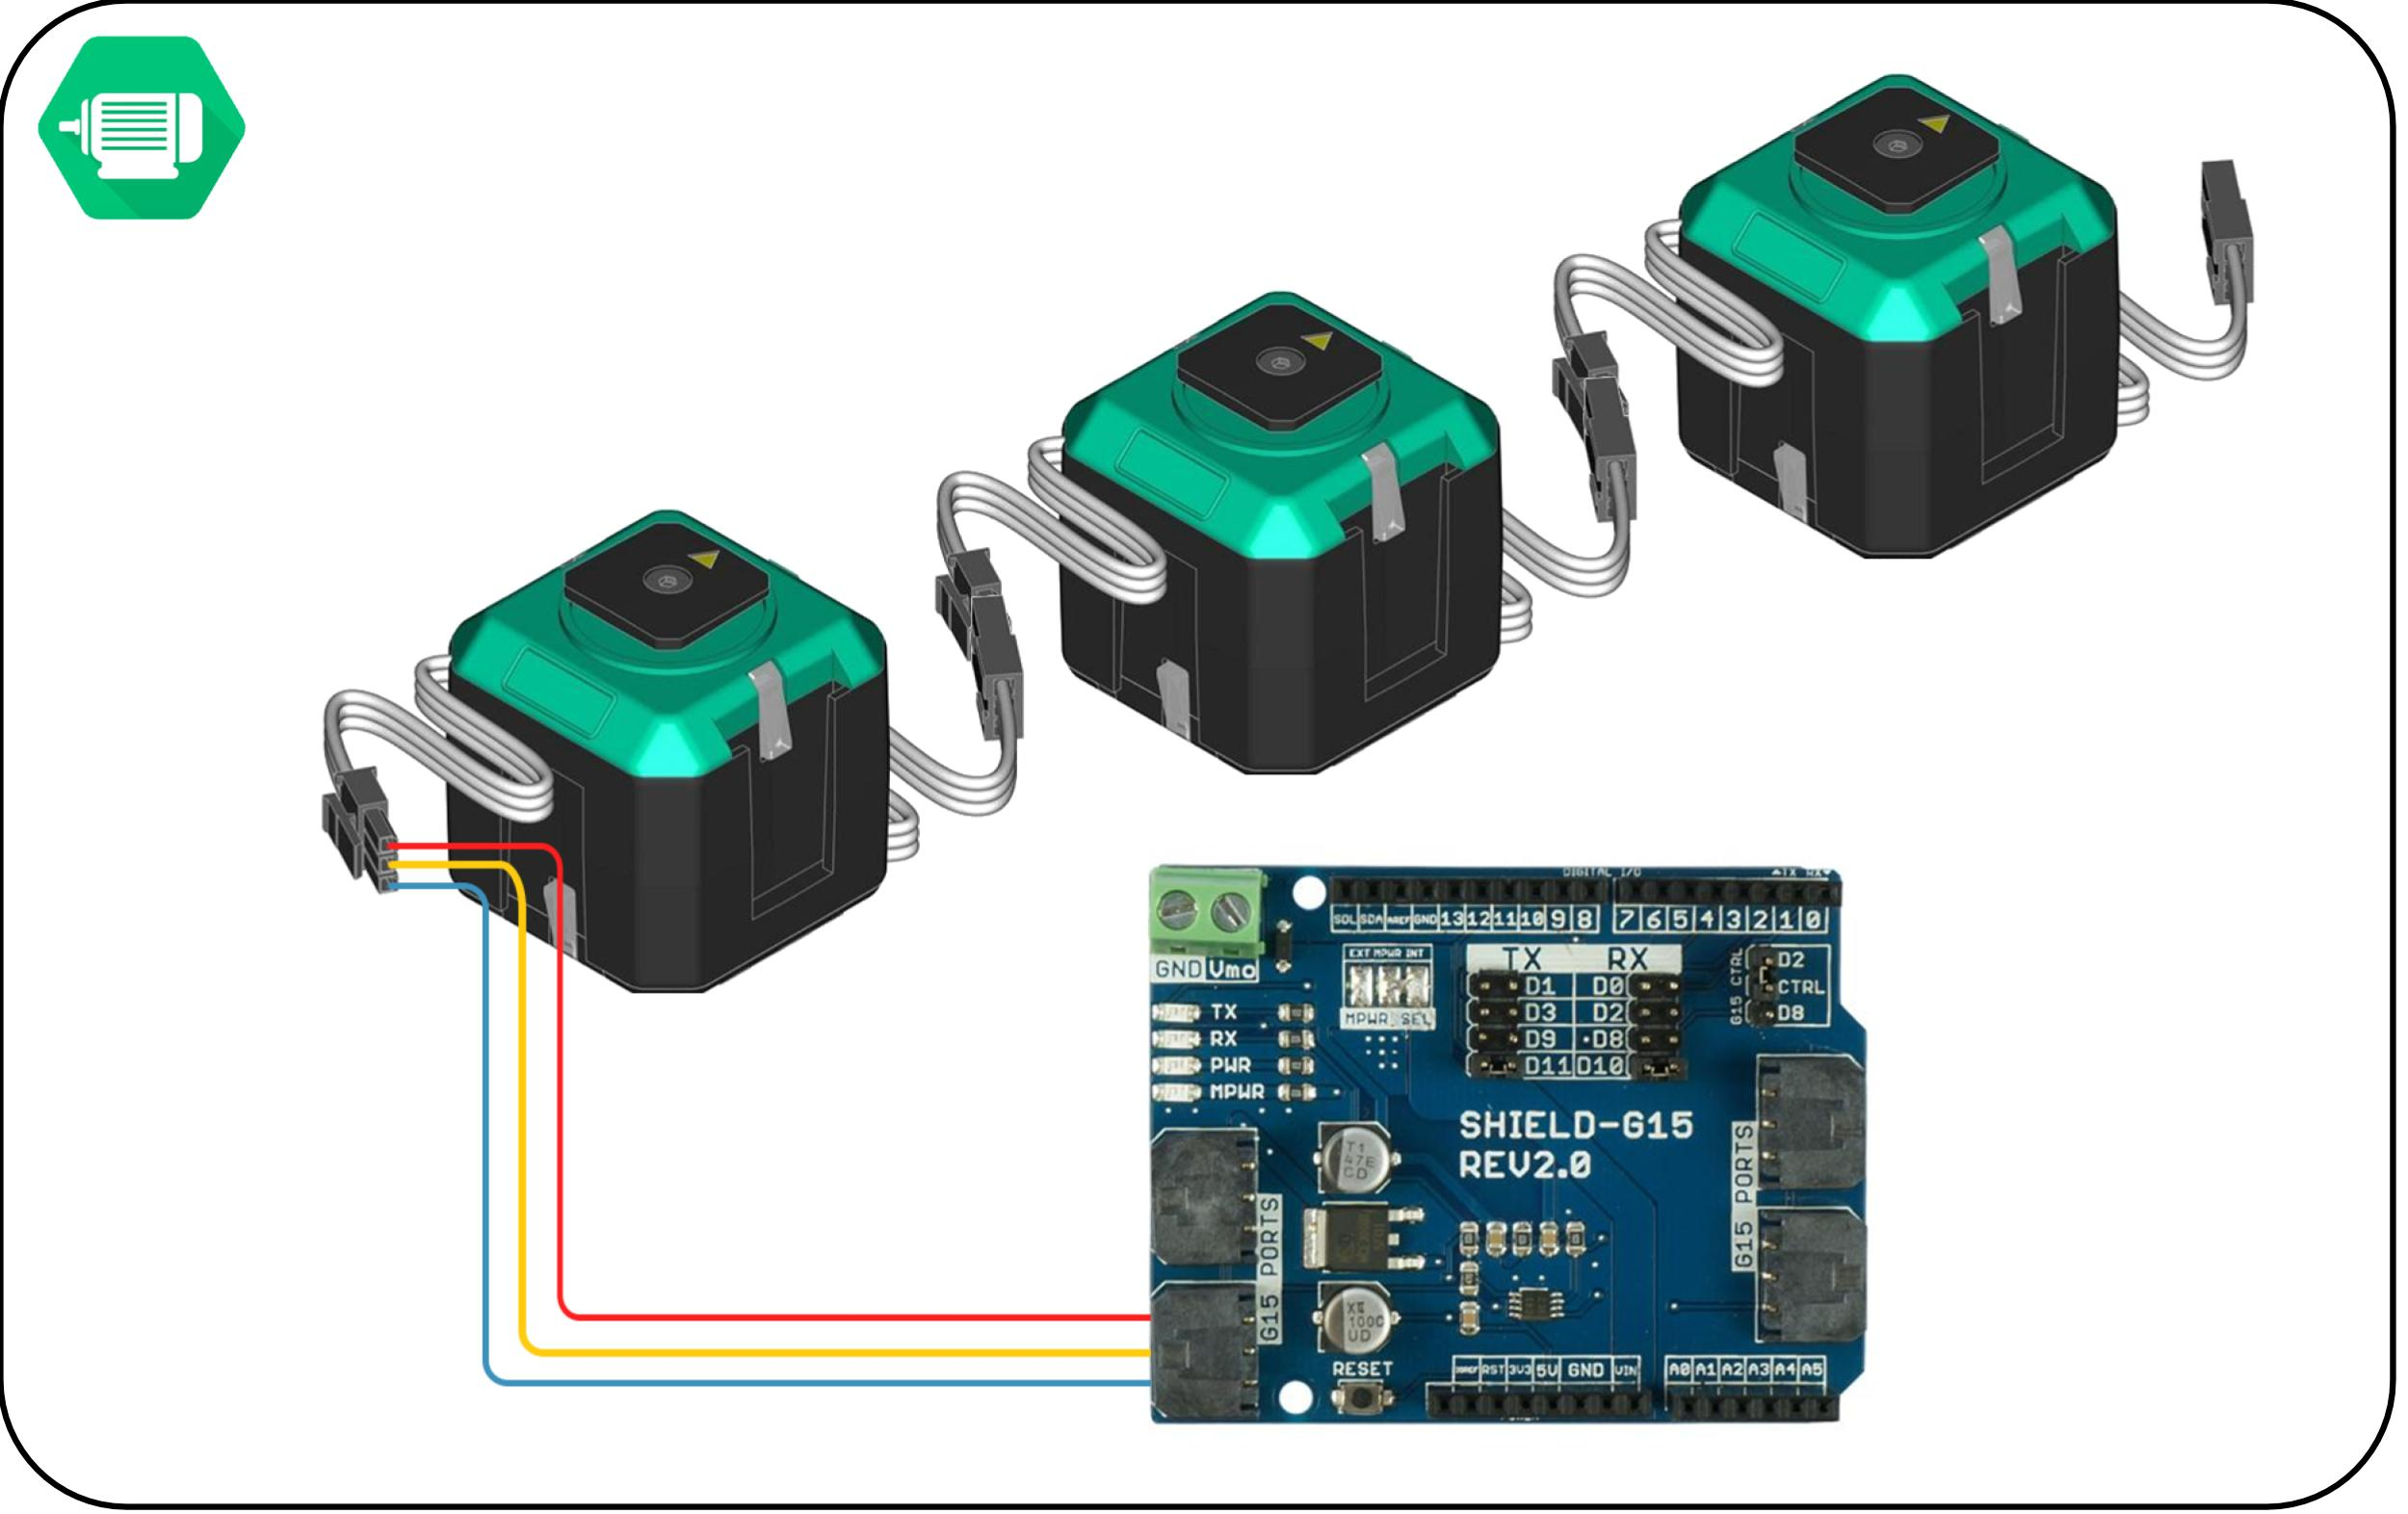
\includegraphics[width=0.8\textwidth]{figuras/Imagenes_Electronica/G15_bus_conection.jpg}
    	\caption{Esquema de la conexión de los servos formando un bus serie de servos y la placa \ingles{Shield}}
    	\label{fig:Electronica:bus-servos}
    	\immagesource{Montaje del Autor a partir de imágenes del fabricante}
    \end{figure}
    
    Para hacer efectiva la comunicación los servos G15 Cube cuentan con dos puertos de tres cambles cada uno. Cada uno cuenta con un conector de aspecto y forma diferente que fuerzan las conexiones en un mismo sentido siempre de forma inequívoca. Estos tres cables, como se puede ver en la imagen \ref{fig:Electronica:conectores-servos}, son utilizados para alimentación, referencia a tierra y canal de información.
    \\
    
    \begin{figure}[H]
    	\centering
    	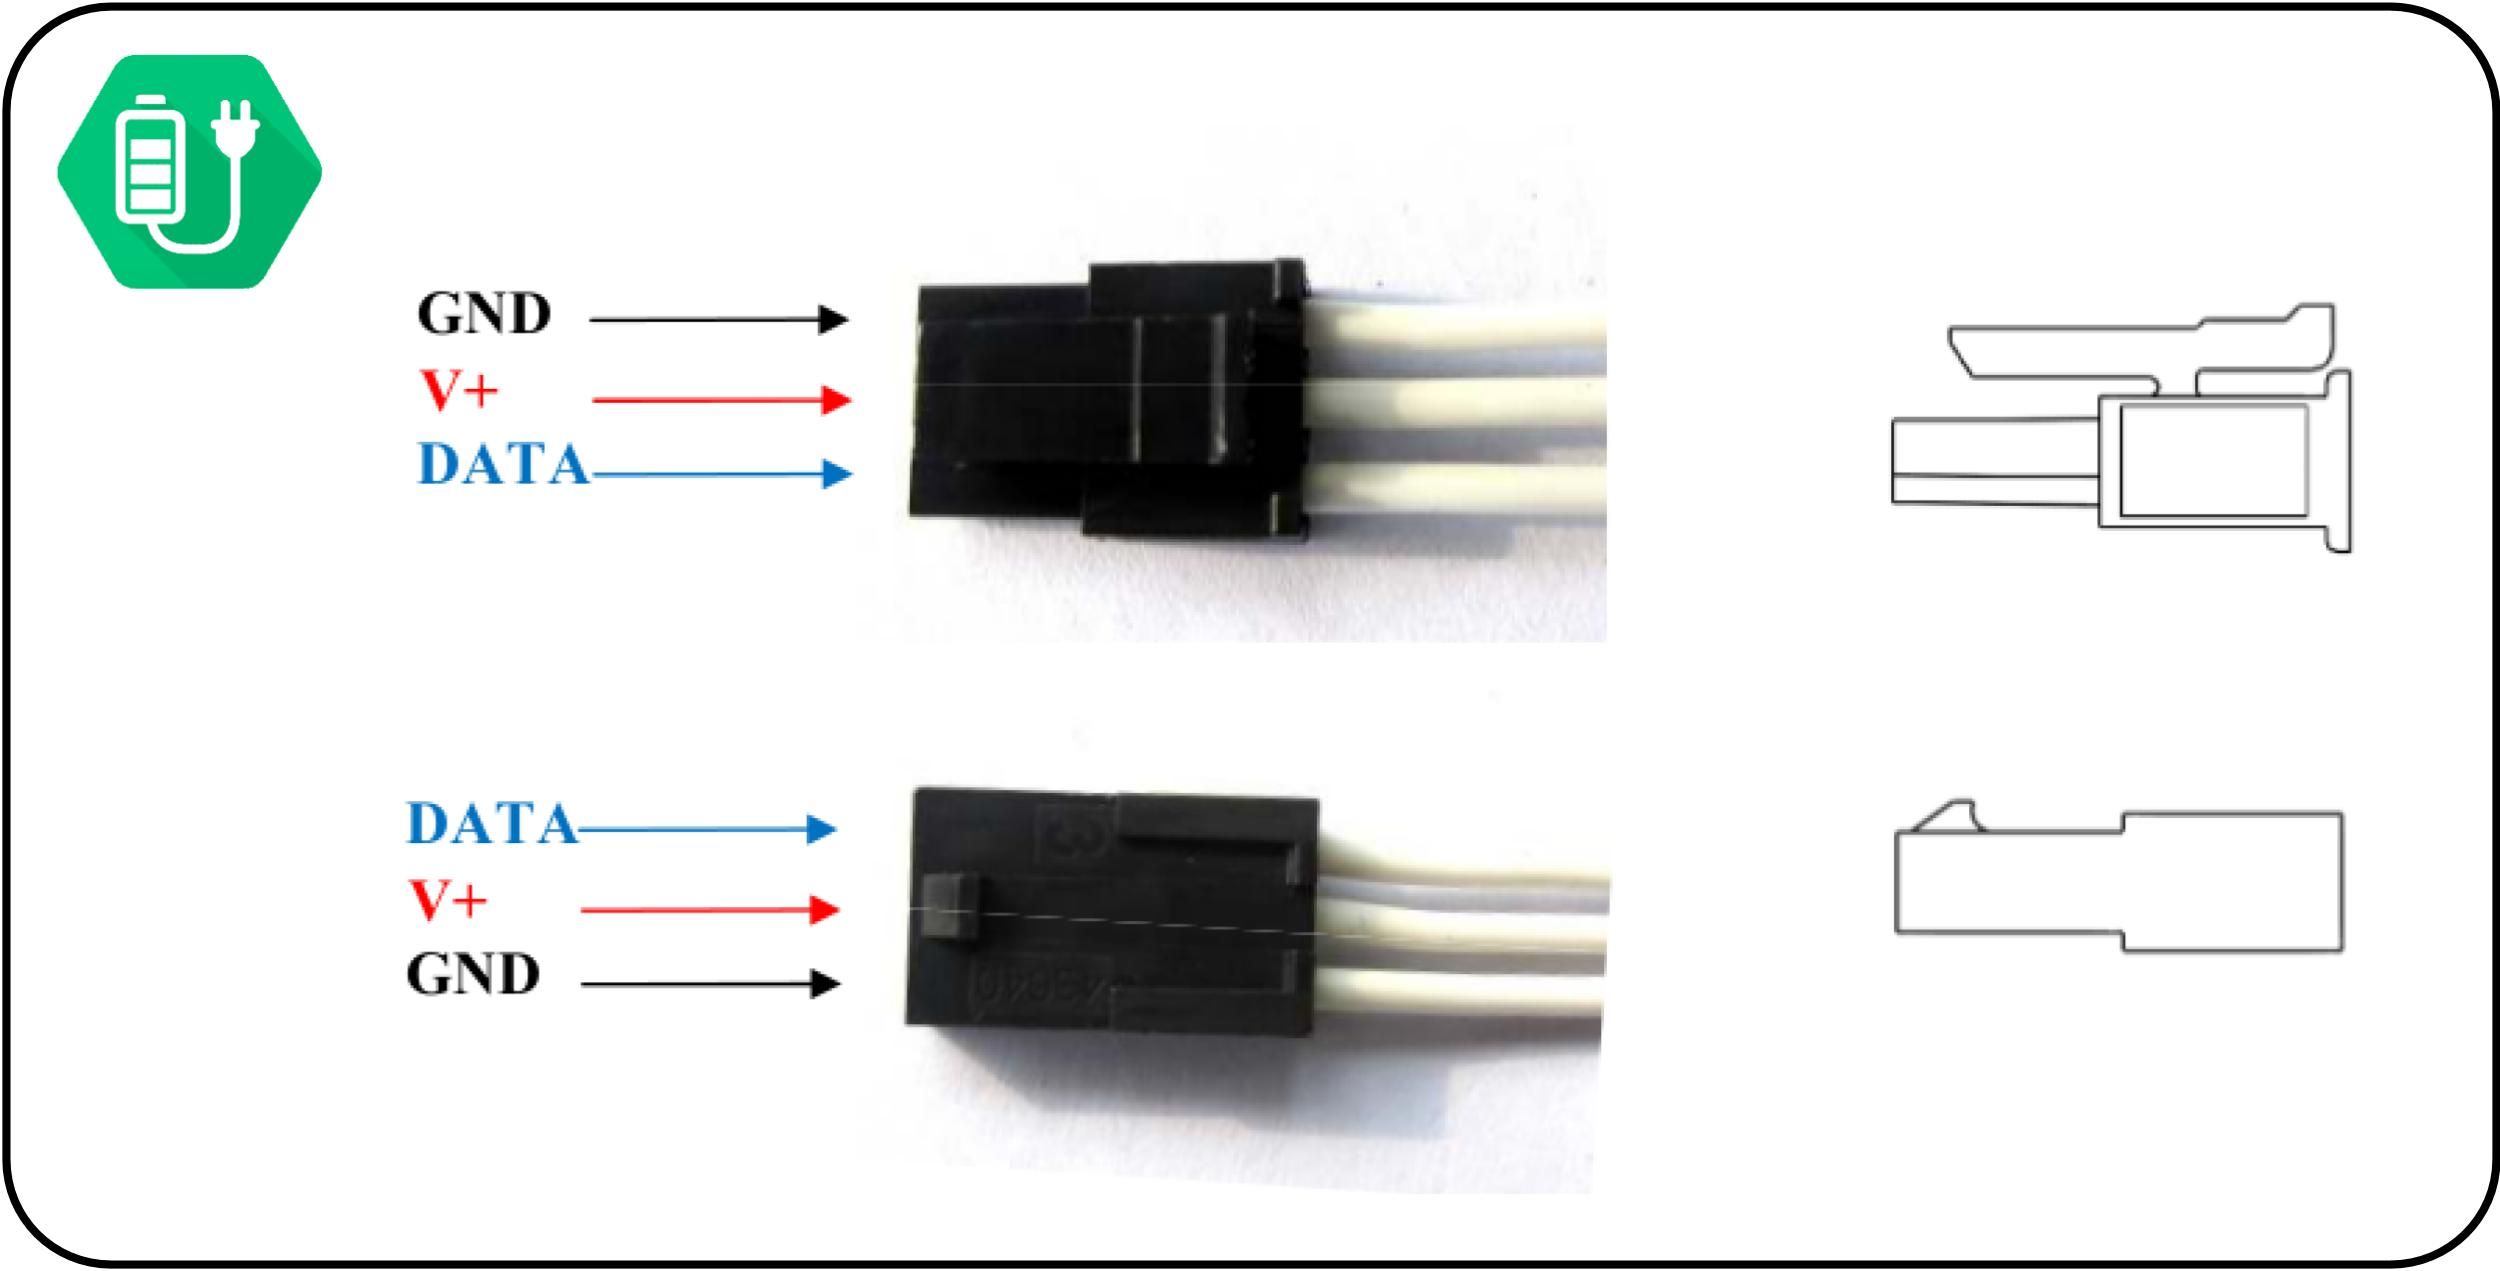
\includegraphics[width=0.7\textwidth]{figuras/Imagenes_Electronica/conectores_servos.jpg}
    	\caption{Conectores de los G15 Cube y uso de cada uno de los cables}
    	\label{fig:Electronica:conectores-servos}
    	\immagesource{Captura obtenida de \cite{CytronTechnologies2012}}
    \end{figure}
    
    Entre las ventajas de utilizar \glosarioPlural{smartservo} es que se cuenta con información relevante que se podrá \textit{preguntar} al servo cuando sea necesaria. Estos servos tienen diferentes modos de funcionamiento, aunque se utilizará principalmente el modo de \textbf{giro continuo}. Para este caso los servos ofrecen un control en par de manera que se podrán enviar comandos del par que deberá ejercer. Como información relevante a consultar ofrece datos de posición del servo, par realizado y sentido del mismo, temperatura, voltaje de alimentación, velocidad y sentido de movimiento, entre otros.
    \\
    
    Cabe destacar algunas características importantes de los mismos, que se encuentran resumidas en la tabla \ref{tab:g15_catact}. Concretamente es de destacar los $12kg \cdot cm$ de par efectivo; un par relativamente bajo que se aprovechará como medida extra de protección a usuarios del brazo robótico tal y como se ha anticipado en capítulos anteriores.

    \begin{table}[H]
    	\caption{Características relevantes de los Servos G15 de Cytron.}
    	\immagesource{Tabla traducida y resumida de \cite{CytronTechnologies2012}}
    	\label{tab:g15_catact}
   		\begin{minipage}{0.42\textwidth}
   		\begin{center}
   		\begin{tabular}{ |c|c|c|c| }
			\hline
			\multicolumn{4}{|c|}{\textbf{Características eléctricas}} \\
			\hline
			\textbf{Parámetro} & \textbf{Valor Mínimo} & \textbf{Valor Típico} & \textbf{Valor Máximo} \\
			\hline
			Voltaje & $6.5V$ & $12V$ & $17.8V$ \\
			\hline
			Consumo de corriente ($12V$) & & & $1.5A$ \\
			\hline
			Temperatura de funcionamiento & $0^oC$ & & $80^oC$ \\
			\hline
			\multicolumn{4}{c}{\textbf{}} \\
			\hline
			\multicolumn{4}{|c|}{\textbf{Especificaciones técnicas}} \\
			\hline
			\multicolumn{2}{|c|}{Peso} & \multicolumn{2}{|c|}{$63g$}\\
			\hline
			\multicolumn{2}{|c|}{Par capaz de realizar (a $12V$)} & \multicolumn{2}{|c|}{$12kg \cdot cm$}\\
			\hline
			\multicolumn{2}{|c|}{Par capaz de soportar} & \multicolumn{2}{|c|}{$15km \cdot cm$} \\
			\hline
			\multicolumn{2}{|c|}{Margen angular de operación } & \multicolumn{2}{|c|}{$360^o$ en giro continuo}\\
			\hline
			\multicolumn{2}{|c|}{Máxima velocidad (en vacío a $12V$)} & \multicolumn{2}{|c|}{$63 RPM$ }\\
			\hline
			\multicolumn{2}{|c|}{Comunicaciçon} & \multicolumn{2}{|c|}{ \begin{minipage}{1.0\textwidth}\vspace{0.1cm}
			Half duplex asynchronous serial \\ communication ($7812.5bps-500kbps $)\end{minipage} }\\
    		\hline
    	\end{tabular}
   		\end{center}
   		\end{minipage}
    \end{table}

\section{Interfaz servos-microcontrolador} \label{sec:Electronica:Potencia}

	Pasada la descripción de los actuadores, los G15 Cube Servo, se hace patente la necesidad de una etapa intermedia entre la placa controladora y los servos que gestione la comunicación entre ambos de forma segura y que desacople la alimentación del controlador de la alimentación de los servos, que requieren un voltaje de 12V (ver \ref{tab:g15_catact}).
	\\
	
	Es la propia marca que fabrica los servos, Cytron Technologies, la que suministra una placa auxiliar o \ingles{shield} con este propósito. Concretamente se utilizará la segunda generación de dicha placa, vista en la figura \ref{fig:Electronica:bus-servos} de la sección anterior.
	\\
	
	Para la alimentación de los servos se ofrecen dos posibles entradas remarcadas en la figura \ref{fig:Electronica:alimentacion-shield} con los colores azul y rojo. Para alternar de una a otra habrá que, mediante el uso de un soldador, modificar la conexión recuadrada en amarillo para habilitar la opción deseada deshabilitando la contraria.
	\begin{itemize}
		\item Alimentación externa (recuadrada en azul): en este caso se conecta la fuente de alimentación directamente a los conectores pasando el voltaje a los cables de alimentación de los servos.
		\item Alimentación mixta shield-controlador (recuadrada en rojo): en este caso la alimentación se comparte con la placa controladora (que deberá rectificar el voltaje de entrada a valores aceptables para la misma). Por defecto esta es la entrada que viene habilitada; se ha mantenido ya que permite la alimentación simultánea de los servos y de la placa controladora a partir de la misma fuente de alimentación (se verá en secciones posteriores la elección del controlador y otros aspectos). 
	\end{itemize}
		
	\begin{figure}[H]
		\centering
		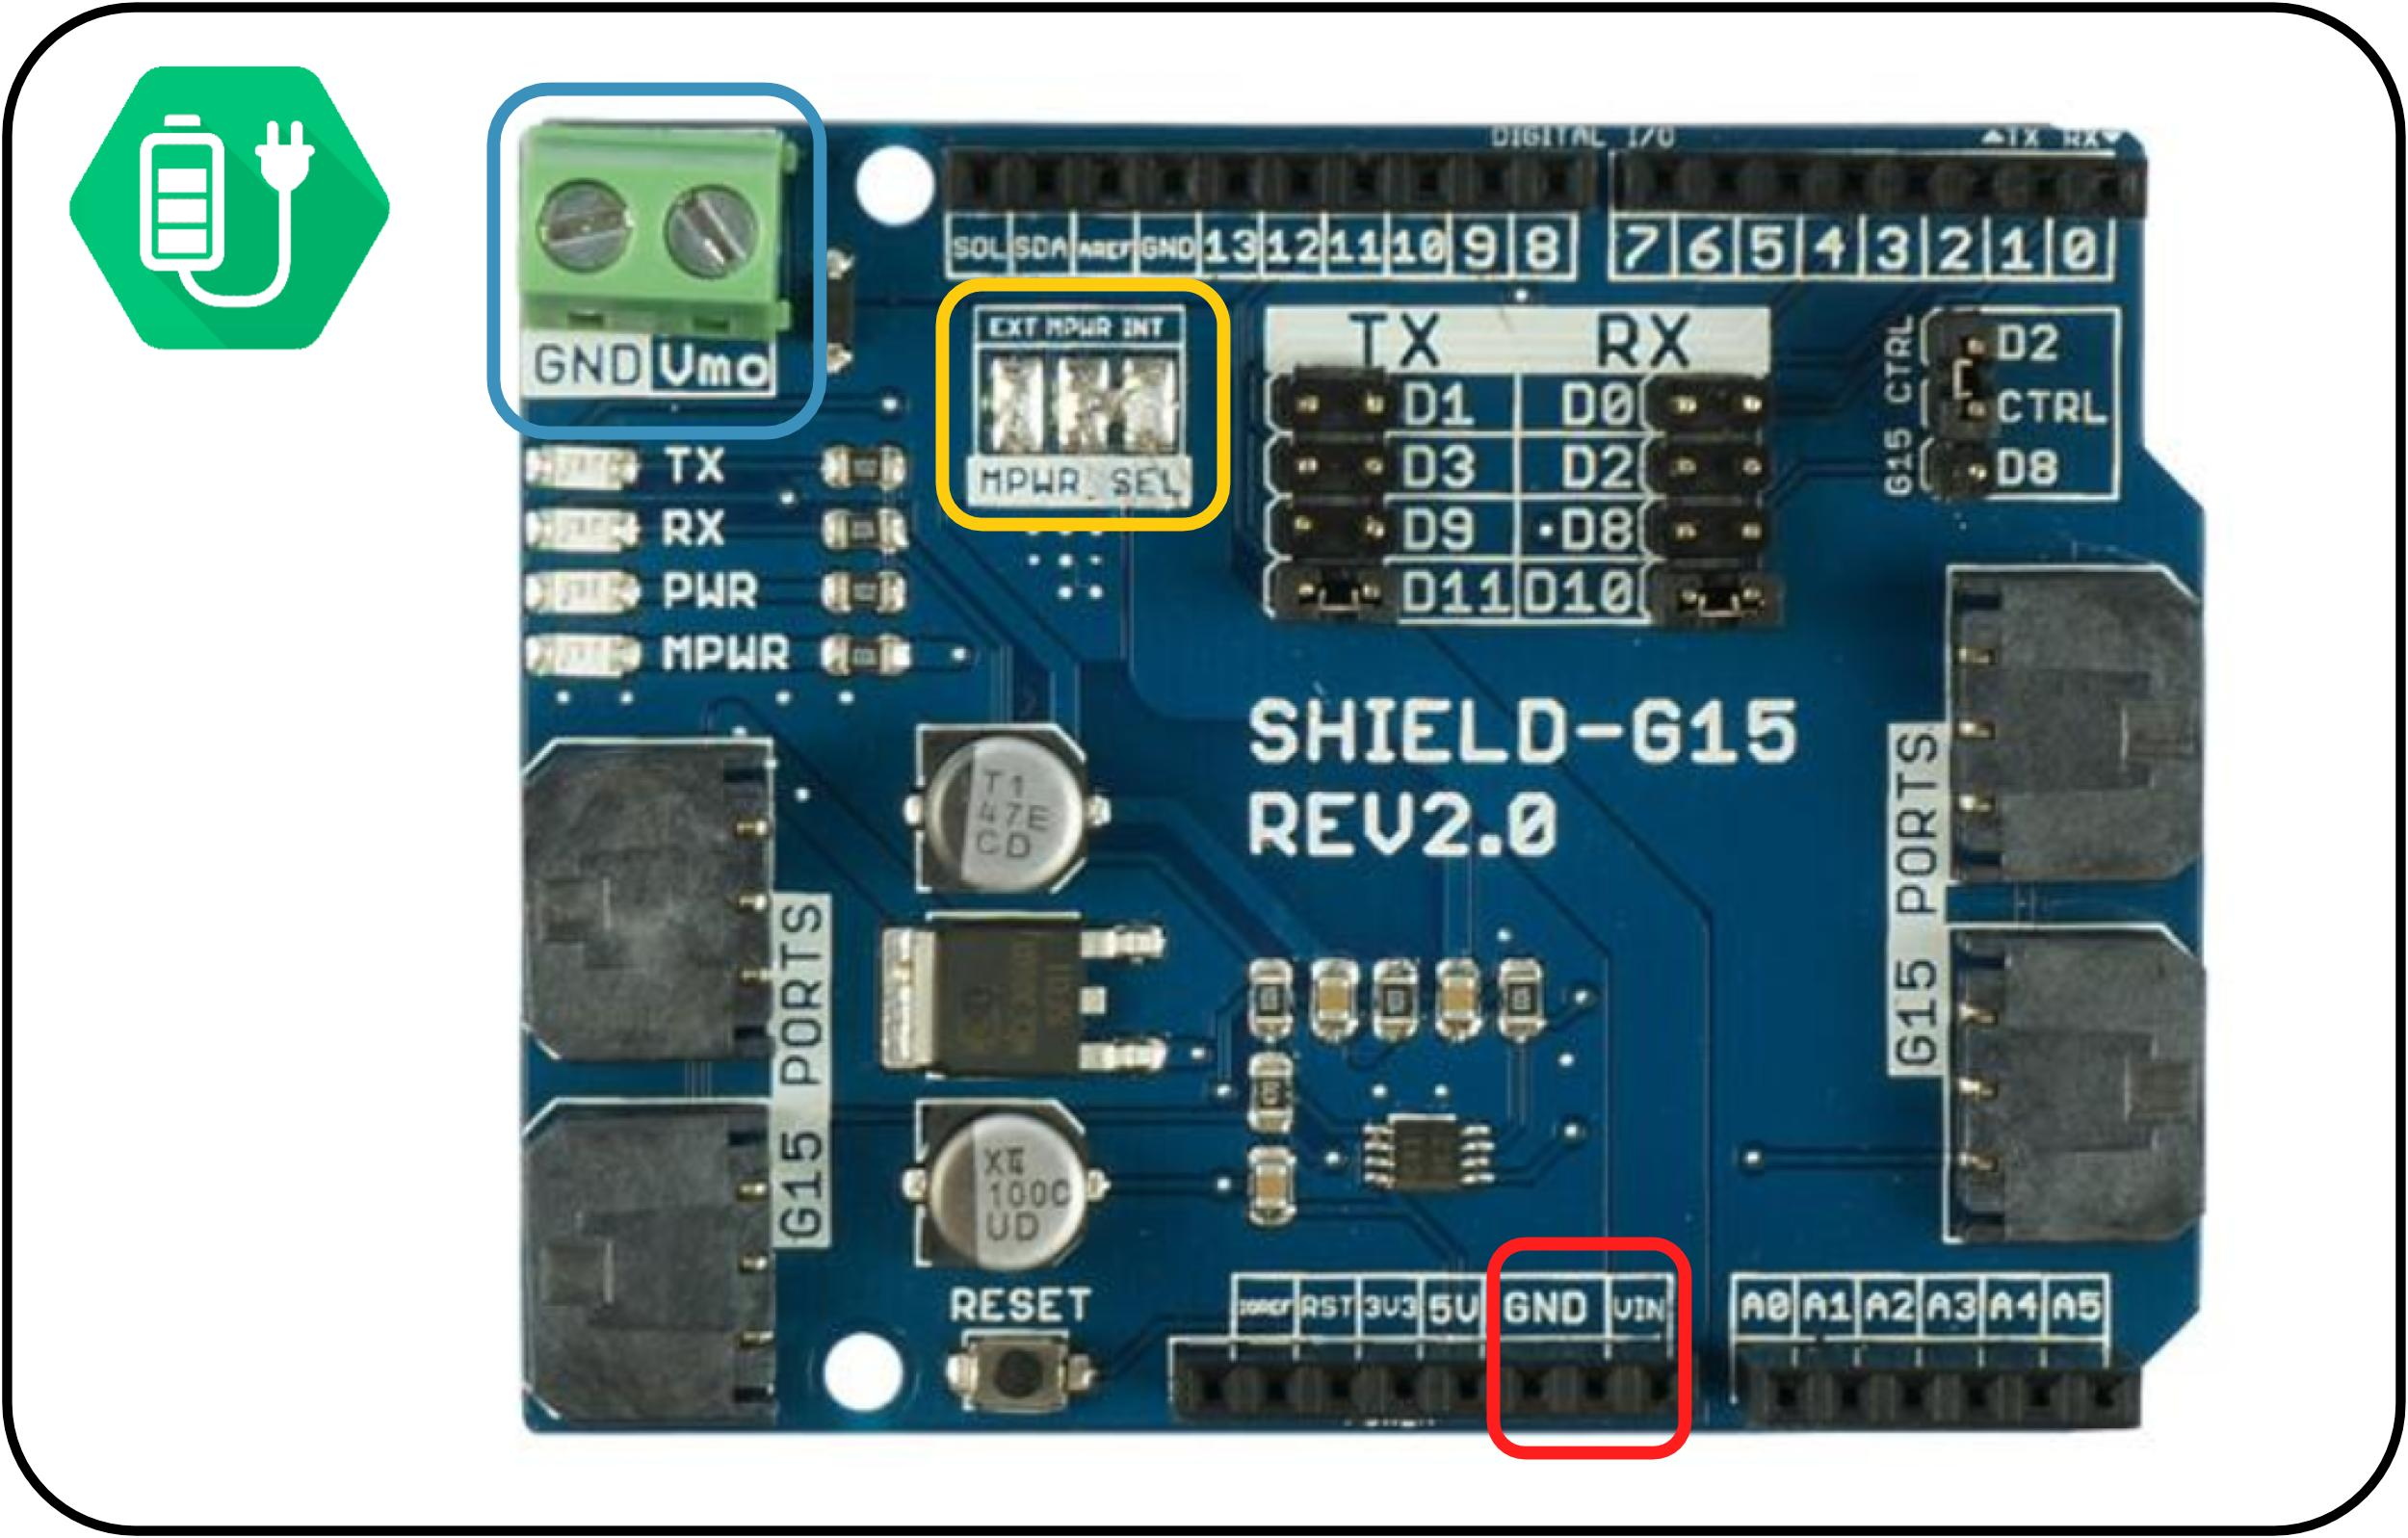
\includegraphics[width=0.7\textwidth]{figuras/Imagenes_Electronica/alimentacion-shield.jpg}
		\caption{Posibilidades para la alimentación de los servos}
		\label{fig:Electronica:alimentacion-shield}
		\immagesource{Captura obtenida de \cite{CytronTechnologies2012} y editada por el Autor del proyecto}
	\end{figure}
		
	En la figura \ref{fig:Electronica:alimentacion-shield} pueden distinguirse una serie de pines de conexión con las letras RX, TX y CTRL. Esta placa está pensada para funcionar a modo de interfaz entre un puerto serie común (con un cable de emisión y otro de recepción de datos) y un puerto serie de tipo \ingles{Half Duplex} como el empleado por los servos.
	\\
	
	Como se describe en \cite{CytronTechnologies2012} la \ingles{shield} incluye integrada un circuito integrado (concretamente el 74HC126 IC) que resuelve los problemas de comunicación inherentes a la comunicación bidireccional por un solo hilo. A través de un pin de control (CTRL en la shield) se gestiona la conexión entre el hilo del \ingles{Half Duplex} y los hilos del puerto serie alternando de uno a otro en función del estado de la señal de control (alto nivel o bajo nivel).
	
\section{Placa controladora}
	
	La placa \ingles{shield} descrita en el apartado anterior está especialmente diseñada para encajar en placas tipo Arduino, concretamente el modelo Arduino Uno. En el marco de este proyecto se ha realizado una fase del desarrollo utilizando como base una placa Arduino Uno, aunque posteriormente se ha cambiado a un Arduino Mega. Más adelante se explicará la motivación de dicho cambio, pero merece volver sobre el aspecto de la alimentación de la placa descrito en el apartado anterior. Según se especifica en \cite{arduinoUno} y en \cite{arduinoMega} el voltaje de entrada recomendado abarca desde los 7 a los 12V teniendo como limitación inferior un mínimo de 6V y un máximo de 20V. En este caso se aplicarán 12V, que quedan incluidos dentro del rango recomendado por el fabricante.
	\\
	
	En el caso de la placa Arduino Uno la \ingles{shield} viene preparada para encajar sobre la misma. La comunicación con los servos está pensada para efectuarse de dos formas:
	\begin{itemize}
		\item A través de un puerto serie UART hardware: en el caso de la placa Arduino Uno solo dispone del puerto conectado a los pines 0 y 1, que también es el usado para la carga de software y comunicación con el ordenador, por lo que queda descartado.
		\item Emulando un puerto serie mediante software en otros pines de la placa. La \ingles{shield} trae una serie de \ingles{jumpers} \completarCon{¿Definir o no es necesario?} que permiten cambiar entre una selección de pines para cada caso (RX, TX o CTRL).
	\end{itemize}
	
	Como se puede ver, utilizando una placa Arduino Uno la comunicación con los servos queda relegada a un puerto emulado por software. Esta es la razón principal por la cual se decide cambiar y utilizar una Placa Arduino Mega2560, que además presenta mayores prestaciones respecto a memoria (ver tabla \ref{tab:arduino_comparison}). Para el control del brazo robótico y el diseño y testeo del software es necesario optimizar la velocidad de comunicación entre los dispositivos al máximo. La placa Arduino Mega incluye tres puertos serie hardware adicionales que se podrán puentear a la placa \ingles{shield} para ser utilizados. Esta conexión se puede ver en la figura \ref{fig:Electronica:shield-arduino}. De esta forma se podrá aprovechar todo el potencial de la comunicación a través de un puerto serie hardware. 
	\\
	
	Para hacerse una idea de la importancia que tiene este cambio se ha forzado la comunicación en ambos casos para obtener los máximos en los cuales sería viable trabajar. Los datos presentados en la tabla \ref{tab:comunication_serial} se han obtenido de forma experimental bajo el marco de este proyecto. Entre los mismos se puede apreciar la gran diferencia existente entre las diferentes formas de comunicación. Las velocidades se han ido duplicando (a modo de convencionalismo las velocidades de comunicación estándar para Placas Arduino suelen obtenerse de esta manera) hasta llegar al máximo que permite una comunicación satisfactoria.
	
	 \begin{table}[H]
	 	\caption{Comparativa entre placas Arduino Uno y Arduino Mega2560}
	 	\immagesource{Tabla con información resumida de \cite{arduinoUno} y \cite{arduinoMega} }
	 	\label{tab:comunication_serial}
	 		\begin{center}
	 			\begin{tabular}{ |c|c|c| }
	 				\hline
	 				\textbf{Tipo de comunicación}& \begin{minipage}{.30\linewidth} \textbf{Velocidad máxima  en baudios}  \end{minipage}& \begin{minipage}{.30\linewidth} \textbf{Velocidad máxima en bytes/milisegundo} \end{minipage} \\
	 				\hline
	 				\begin{minipage}{.30\linewidth}\vspace{2pt} Puerto Serie \textbf{Sowtware} (AUno):  Shield-controlador \vspace{2pt} \end{minipage} & 57600 bauds & 7.2 bytes/ms \\
	 				\hline
	 				\begin{minipage}{.30\linewidth}\vspace{2pt} Puerto Serie \textbf{Hardware} (AMega):  Shield-controlador \vspace{2pt} \end{minipage} & 460800 bauds & 57.6 bytes/ms \\
	 				\hline
	 				\begin{minipage}{.30\linewidth}\vspace{2pt} Puerto Serie \textbf{Hardware} (Ambas):  controlador-ordenador \vspace{2pt} \end{minipage} & 921600 bauds & 115.2 bytes/ms \\
	 				\hline
	 			\end{tabular}
	 		\end{center}
	 \end{table}
	 
	 En este proyecto concreto se enlazaran diferentes lazos de control a diferentes frecuencias de refresco (ver capítulo \ref{chap:Control}) que exigirán el máximo de la capacidad comunicativa entre los dispositivos. Los datos máximos obtenidos para la placa Arduino Mega son los utilizados para el funcionamiento del robot.
	
    \begin{figure}[H]
    	\centering
    	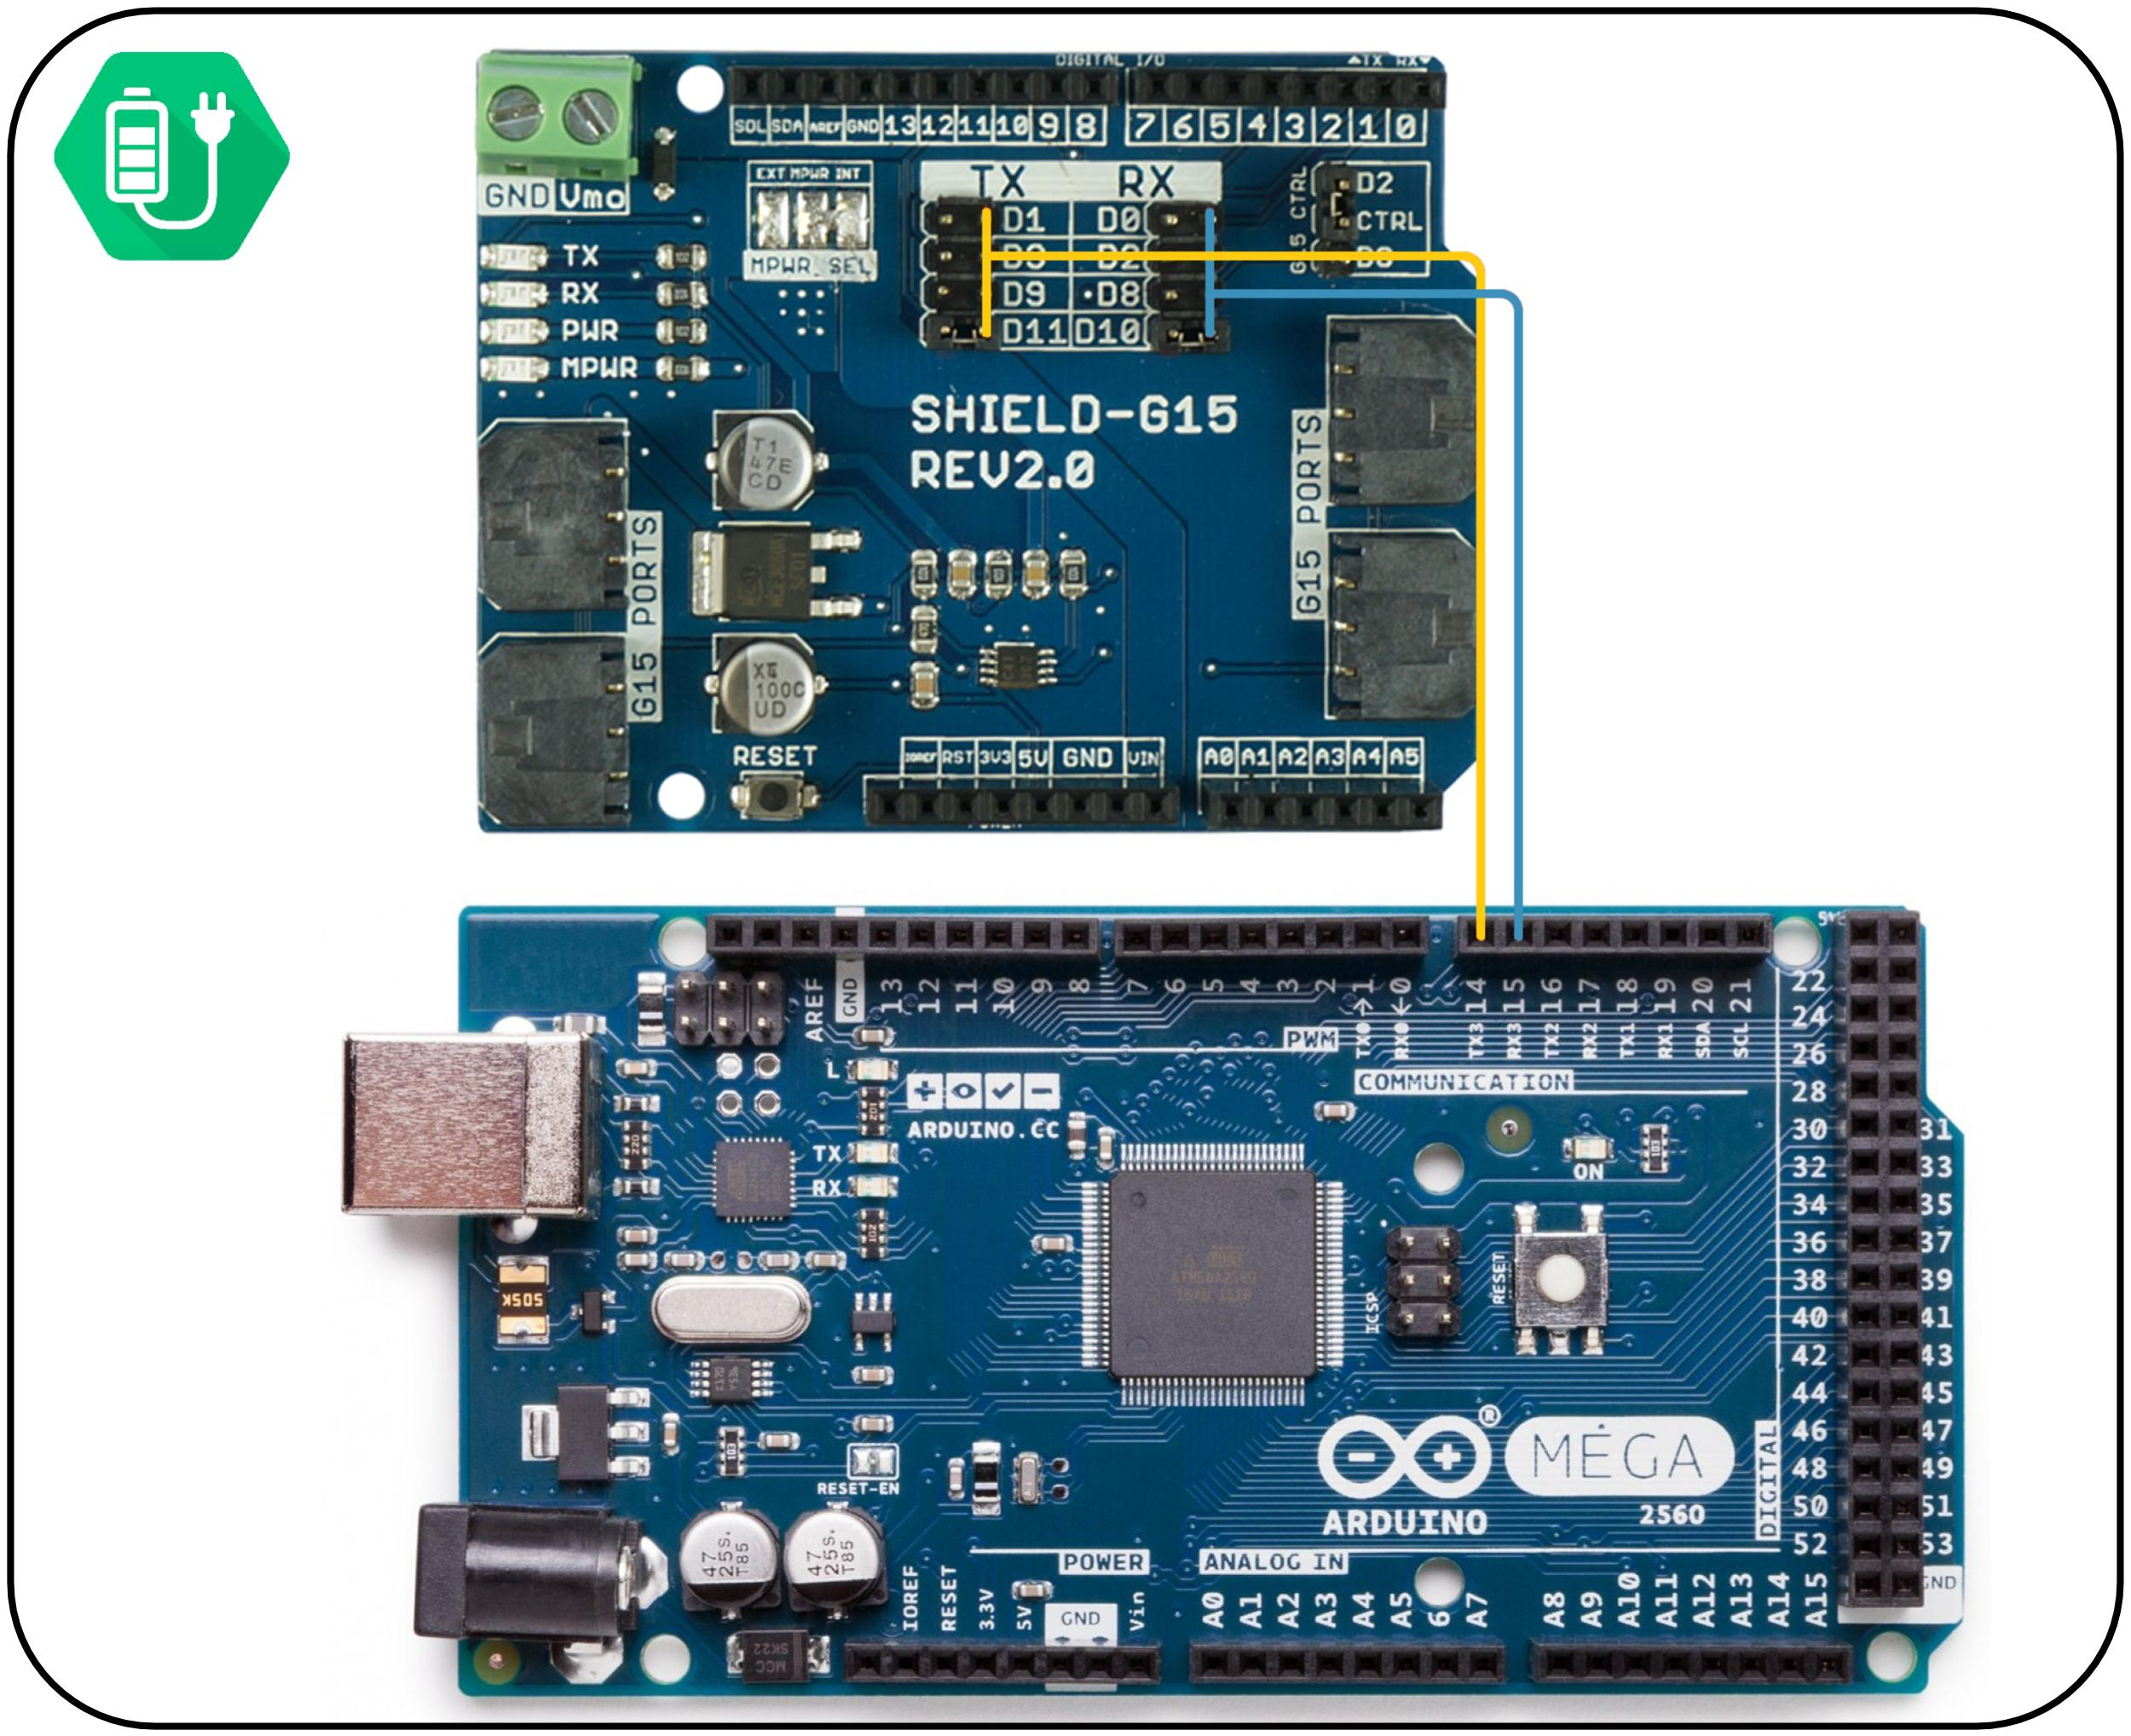
\includegraphics[width=0.75\textwidth]{figuras/Imagenes_Electronica/Shield-Arduino-Conection.jpg}
    	\caption{Esquema de la conexión entre la placa Shield y Arduino para utilizar los puertos Hardware Serie de la Arduino Mega}
    	\label{fig:Electronica:shield-arduino}
    	\immagesource{Montaje del Autor a partir de imágenes del fabricante}
    \end{figure}
    
    \begin{table}[H]
       	\caption{Comparativa entre placas Arduino Uno y Arduino Mega2560}
       	\immagesource{Tabla con información resumida de \cite{arduinoUno} y \cite{arduinoMega}}
       	\label{tab:arduino_comparison}
       	%\begin{minipage}{0.42\textwidth}
       		\begin{center}
       			\begin{tabular}{ |c|c|c| }
       				\hline
       				&\textbf{Arduino Uno}&\textbf{Arduino Mega2560} \\
       				\hline
       				Número de pines entrada/salida & 14 & 54 \\
       				\hline
       				Memoria flash & 32KB & 256 KB \\
       				\hline
       				SRAM & 2KB & 8KB \\
       				\hline
       				EEPROM & 1KB & 4KB \\
       				\hline
       				Velocidad de reloj & 16MHz & 16Mhz \\
       				\hline
       			\end{tabular}
       		\end{center}
       	%\end{minipage}
    \end{table}

\section{Sensores} \label{sec:Electronica:Sensores}


 \chapter{Software involucrado en el proyecto} \label{chap:SW}
\hrule
\vspace{3mm}

    En este capítulo se hace una descripción detallada del \ingles{software} involucrado en este proyecto. Primeramente se hace un repaso de la estructura de directorios, que es característica y viene previamente marcada por el software utilizado. Una vez explicado se pasará a describir las diferentes librerías que se han desarrollado (sección \ref{sec:SW:lib}) y del directorio de fuentes principal SRC (sección \ref{sec:SW:src}). Se deja para una sección posterior la interacción e integración de estos objetos así como una explicación más detallada del flujo de la información, funcionamiento del sistema como ejemplos de uso (sección \ref{sec:SW:interacion_informacion_proced}). Finalmente se exponen los test realizados sobre el software (sección \ref{sec:SW:test}) así como la gestión de la complejidad (sección \ref{sec:SW:gestion_complejidad}) del proyecto.
    \\ 

    Para el desarrollo y test del software se ha utilizado el editor \glosario{Atom} ampliando su funcionalidad con el paquete \glosario{PlatformIO}, que expande las capacidades del editor base para permitir trabajar con diferentes placas, entre ellas las de la gama de \glosario{Arduino}.
    \\ 
    
    La elección de esta herramienta conlleva un formato en el árbol de directorios en los que se separa el código determinado. Concretamente queda de la siguiente manera:

    \lstset{language=C, breaklines=true, basicstyle=\footnotesize}
        %Introducir label y caption
        \begin{lstlisting}[frame=single]
        
     -- Sw
     |-- lib
     |  |-- debug
     |  |-- joint_handler
     |  |-- joint_rha
     |  |-- rha_types
     |  |-- servo_rha
     |  |-- readme.txt
     |-- src  
     |  |-- main.cpp
     |  |-- utilities.cpp
     |  |-- utilities.h
     |-- test
     |  |-- test_cytrong_g15_servo
     |  |-- test_servo_mock
     |  |-- test_servo_real
     |-- platformio.ini
     -------
     |-- code_analysis
     |-- makeAnalysis.sh
        \end{lstlisting}
    
    En los siguientes apartados se hará un análisis detallado del contenido de estos directorios. Se desarrollan primero los ficheros con información auxiliar y posteriormente en una jerarquía desde más afuera \textcolor{pRojo}{$<$---- ¿?¿W T F?¿?} detallando luego los componentes internos.
\section{Librerías (directorio lib)} \label{sec:SW:lib}

    \subsection{debug} \label{subsec:SW:lib:debug}
        Dentro de este directorio se encuentra el fichero debug.h donde se han definido macros para \glosario{debug} de los diferentes espacios. A continuación se muestra un ejemplo de como se codifican dichas macros para hacer un seguimiento de la clase \ingles{servo\_rha} (Ver apartado \ref{subsec:SW:lib:servo_rha}).
        
        \lstset{language=C, breaklines=true, basicstyle=\footnotesize}
        %Introducir label y captio
        \begin{lstlisting}[frame=single]
        
    #ifdef DEBUG_SERVO_RHA
        #define DebugSerialSRHALn(a) {  Serial.print("[DC]  ServoRHA::"); Serial.println(a); }
        #define DebugSerialSRHALn2(a, b) {  Serial.print("[DC]  ServoRHA::"); Serial.print(a); Serial.println(b); }
        #define DebugSerialSRHALn4(a, b, c, d) {  Serial.print("[DC]  ServoRHA::"); Serial.print(a); Serial.print(b); Serial.print(c); Serial.println(d); }
    #else
        #define DebugSerialSRHALn(a)
        #define DebugSerialSRHALn2(a, b)
        #define DebugSerialSRHALn4(a, b, c, d)
    #endif
            
        \end{lstlisting}

        Como se puede apreciar estas macros utilizan la comunicación serial de \glosario{Arduino}, concretamente la función \ingles{print} y \ingles{println} de la librería \ingles{Serial} para mostrar los mensajes en un formato determinado. Además se definen de tal forma que se pueden activar o desactivar (en este mismo fichero \ingles{debug.h}) de forma que se enviarán o no los mensajes de \glosario{debug}. A través de este tipo de mensajes se puede hacer un seguimiento de la ejecución de los diferentes métodos o funciones de la librería afectada para ubicar fallos en los mismos.

        Para activar la opción de \glosario{debug} bastará con descomentar la línea correspondiente:

        \lstset{language=C, breaklines=true, basicstyle=\footnotesize}
        %Introducir label y captio
        \begin{lstlisting}[frame=single]
        
    // #define DEBUG_SERVO_RHA
    // #define DEBUG_TEST_SERVO_RHA_MOCK
    #define DEBUG_TEST_SERVO_RHA_REAL
    // #define DEBUG_CYTRON_G15_SERVO
    // #define DEBUG_TEST_CYTRON_G15_SERVO
            
        \end{lstlisting}
        
    \subsection{rha\_types} \label{subsec:SW:lib:rha_types}
        Dentro de este directorio se encuentra el fichero \ingles{rha\_types.h} donde se definen algunos tipos de datos y estructuras que se usan en el proyecto.
        \\
        
        Estas estructuras de datos se listan a continuación, pudiendo ver sus respectivos diagramas de clases en la figura \ref{fig:SW:class_diagram_TRHA}:
        
        \begin{itemize}
            \item \ingles{SpeedGoal} condensa en un solo objeto toda la información necesaria para codificar un objetivo de velocidad.
            \item \ingles{Regulator} encapsula el funcionamiento de un \glosario{Regulador-PID} estandar. Guarda los valores de las constantes así como de la integral del error para luego, pasándole error, derivada del error e integral del error en un intervalo poder devolver la salida del regulador.
            \item \ingles{Timer} codifica un temporizador (en milisegundos) de forma que se le podrá preguntar al objeto si el tiempo ya ha pasado, bloqueando o no la ejecución del programa hasta el final del tiempo.
            \item \ingles{TimerMicroseconds} hereda las características del objeto \ingles{Timer} funcionando en microsegundos.
        
        \end{itemize}
        
        \begin{figure}[H]
            \centering
            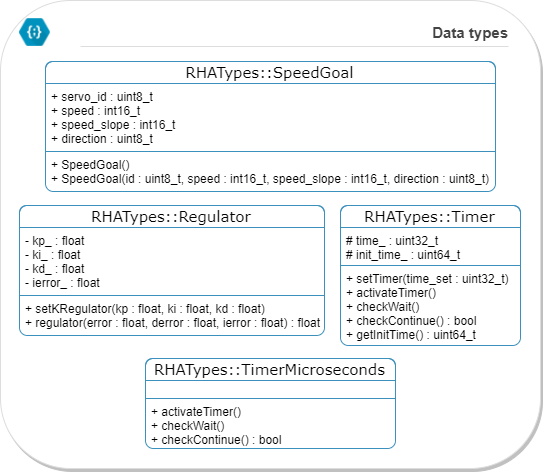
\includegraphics[width=0.8\textwidth]{figuras/SW/class_diagram_TRHA.png}   
            \caption{Estructuras de datos auxiliares}
            \label{fig:SW:class_diagram_TRHA}
        \end{figure}
        
        Se puede consultar información de más bajo nivel referente a estos tipos de datos en el Anexo \ref{app:documentacion_software} sección \completar.
    \subsection{joint\_handler} \label{subsec:SW:lib:joint_handler}
        La librería \ingles{joint\_handler} se hace cargo de generar un objeto de la clase \ingles{JointHandler} que será en encargado de gestionar la sincronización de todas las articulaciones. Este objeto es propietario de las articulaciones e implementa un método que cíclicamente sincroniza el funcionamiento de todas las articulaciones. En el objeto \ingles{JointHandler} se implementa a su vez la comunicación con los \glosarioPlural{servo}, es decir, el encapsulamiento de los paquetes de datos con la información genérica de forma que la información que se envía cumpla con el protocolo de comunicación que comparten los \glosarioPlural{servo}. Además implementa las funciones que gestionan el envío y recepción de dichos paquetes de datos.
        
        El bucle de control implementado se encarga de ir llamando una a una a todas las articulaciones para que hagan las siguientes operaciones (se puede ver representado el funcionamiento de dicho ciclo en la Figura \ref{fig:SW:joint_handler_loop}):
        \begin{enumerate}
            \item Asegurar que cada articulación actualice la información propia, compuesta por la posición recibida de la realimentación así como toda la información proveniente del servo (datos de posición, velocidad, par soportado y dirección en que se aplican, voltaje y temperatura).
            \item Llamar a cada articulación para que se realicen los cálculos correspondientes del \ingles{torque} que se enviará calculado a partir del error entre la velocidad real y deseada. Este valor queda guardado en cada servo para ser posteriormente empaquetado.
            \item Invocar a cada servo para que se adhieran al paquete de información que se va a enviar.
            \item Se enpaqueta la información a enviar a los diferentes \glosarioPlural{servo} en un mismo paquete, añadiendo posteriormente el correspondiente encabezado así como el comprobante de que el paquete se ha recibido correctamente (checksum). Una vez preparado el paquete se envía por el puerto serie.
        \end{enumerate}
        
        \begin{figure}[H]
        \centering
        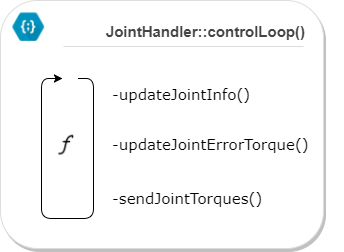
\includegraphics[width=0.45\textwidth]{figuras/SW/joint_handler_loop.png}   
        \caption{Esquema de ejecución de bucle de control de joint\_handler}
        \label{fig:SW:joint_handler_loop}
        \end{figure}
        
        Como se puede intuir es en este objeto donde realmente se implementa el lazo de control de velocidad para todos los \glosarioPlural{servo} conectados al bus. Esta serie de operaciones descrita anteriormente constituye, de forma discretizada, el lazo de control representado en la Figura \ref{fig:SW:servo_control_loop} para cada servo y asegura su correcto funcionamiento y sincronismo.
        
        \begin{figure}[H]
        \centering
        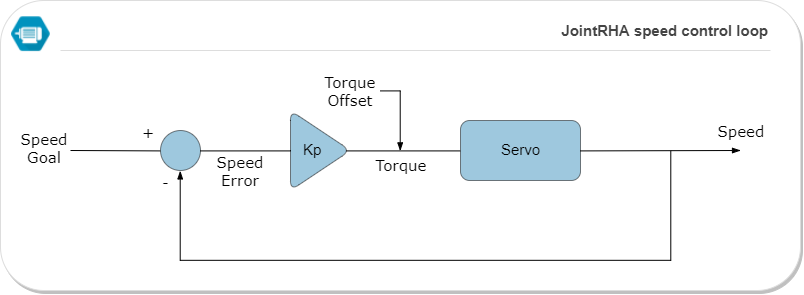
\includegraphics[width=0.85\textwidth]{figuras/SW/servo_control_loop.png}   
        \caption{Lazo de control de la velocidad del servo. Cálculos realizados por el objeto \ingles{ServoRHA}.}
        \label{fig:SW:servo_control_loop}
        \end{figure}
            
        \begin{figure}[H]
            \centering
            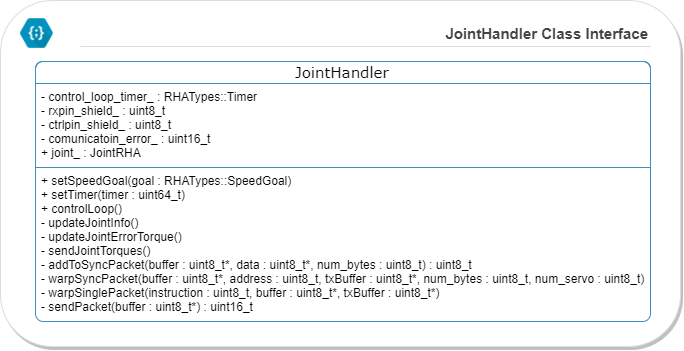
\includegraphics[width=0.95\textwidth]{figuras/SW/class_diagram_JH.png}   
            \caption{Atributos y métodos más relevantes del objeto \textit{JointHandler}}
            \label{fig:SW:class_diagram_JH}
        \end{figure}
        
        Se puede consultar información de más bajo nivel referente al objeto \ingles{JointHandler} así como a sus atributos y métodos en el Anexo \ref{app:documentacion_software} sección \completar.
    
    \subsection{joint\_rha} \label{subsec:SW:lib:joint_rha}
        La librería \ingles{joint\_rha} implementa un objeto de tipo \ingles{JointRHA} que aúna en un mismo objeto las lecturas y capacidades del objeto \ingles{ServoRHA} (explicado en la sección \ref{subsec:SW:lib:servo_rha}) junto con la realimentación de posición de la articulación en cuestión.
        
        \begin{figure}[H]
            \centering
            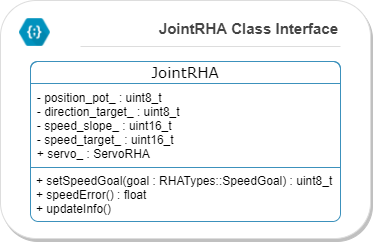
\includegraphics[width=0.5\textwidth]{figuras/SW/class_diagram_JRHA.png}   
            \caption{Atributos y métodos más relevantes del objeto \textit{JointRHA}}
            \label{fig:SW:class_diagram_JRHA}
        \end{figure}
        
        Se puede consultar información de más bajo nivel referente al objeto \ingles{JointRHA} así como a sus atributos y métodos en el Anexo \ref{app:documentacion_software} sección \completar.
        
    \subsection{servo\_rha} \label{subsec:SW:lib:servo_rha}
        La librería \ingles{servo\_rha} implementa un objeto del tipo \ingles{ServoRHA} que está encargado de gestionar toda la información referente al servo. Se encarga de encapsular la información específica a un servo en paquetes de datos a petición del objeto \ingles{JointHandler} que luego serán procesados por el mismo previo a ser enviados a través del bus. Estos paquetes se forman a partir de la información contenida en el objeto \ingles{ServoRHA}, que además de formar los paquetes a enviar almacena la información referente al servo que se recibe de los mismos. 
        \\
        
        Gestiona además una parte importante referente al lazo de control de velocidad del servo vista en el apartado \ref{subsec:SW:lib:joint_handler}. El objeto \ingles{ServoRHA} contiene los datos del regulador utilizado así como el offset a aplicar. De esta forma, recibiendo el error realiza las operaciones para calcular y empaquetar el \ingles{torque} deseado. En la Figura \ref{fig:SW:servo_control_loop_servo_part} se representa, recuadrado, la parte correspondiente del lazo de control de velocidad (representado anteriormente en la Figura \ref{fig:SW:servo_control_loop}) que efectúa el objeto en cuestión.
        \begin{figure}[H]
        \centering
        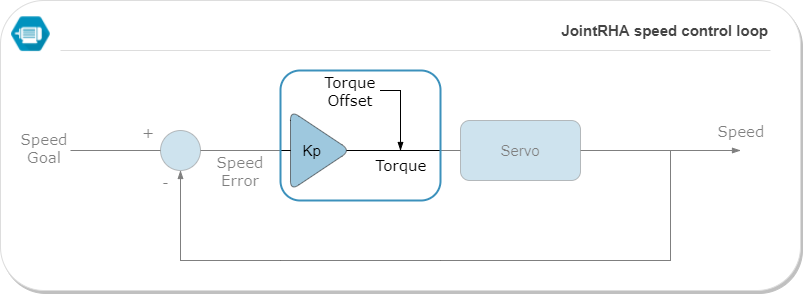
\includegraphics[width=0.85\textwidth]{figuras/SW/servo_control_loop_servo_part.png}   
        \caption{Lazo de control de la velocidad del servo. Cálculos realizados por el objeto \textit{ServoRHA}.}
        \label{fig:SW:servo_control_loop_servo_part}
        \end{figure}
        
        \begin{figure}[H]
            \centering
            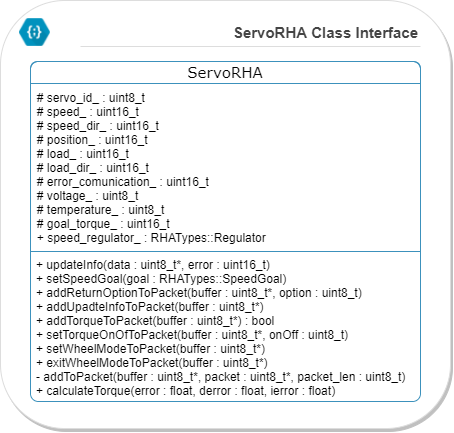
\includegraphics[width=0.65\textwidth]{figuras/SW/class_diagram_SRHA.png}   
            \caption{Atributos y métodos más relevantes del objeto \textit{ServoRHA}}
            \label{fig:SW:class_diagram_SRHA}
        \end{figure}
        
        Se puede consultar información de más bajo nivel referente al objeto \ingles{ServoRHA} así como a sus atributos y métodos en el Anexo \ref{app:documentacion_software} sección \completar.
        
\section{SRC. Fichero de código principal} \label{sec:SW:src}

\section{Interacción entre objetos, flujo de la información y de procedimientos} \label{sec:SW:interacion_informacion_proced}

\section{Test y verificación del software} \label{sec:SW:test}
    Como parte del proyecto se han desarrollado una serie de test para verificar el correcto funcionamiento de las diferentes librerías.

    Para el desarrollo y ejecución de dichos test se ha utilizado la funcionalidad de test que viene integrada en \glosario{PlatformIO}: \glosario{PlatformIO_Test}. Esta herramienta, permite definir una serie de test que pueden ser ejecutados en la propia placa. De esta forma se puede automatizar el proceso de test.

    Una completa definición de test (desde test unitarios hasta test de integración) permite controlar de forma continuada el correcto funcionamiento del sistema frente a modificaciones en el código. De forma genérica estos test se dividen en:

    \begin{itemize}
        \item test\_cytrong\_g15\_servo 
        \item test\_servo\_mock
        \item test\_servo\_real
    \end{itemize}

    El el directorio SW/test se encuentran definidos los diferentes test que se realizan. Cada fichero de test, destinado a testear de forma parcial o completa una librería, tiene diferentes test definidos en formato de función para los diferentes métodos contenidos en la librería.

    Para testear un método o grupo de métodos se define una función de test en la que se define la ejecución que se va a realizar, con las entradas predefinidas de forma que se puede comprobar como ciertas salidas o parámetros internos satisfacen las necesidades impuestas. Para la definición de estas condiciones así como de los test se sigue el formato propuesto desde \glosario{PlatformIO_Test} y la API que adjuntan.


\section{Gestión de la complejidad y mantenibilidad:} \label{sec:SW:gestion_complejidad}
    Para controlar el desarrollo del proyecto de forma paralela en todas sus partes asegurando así un control de la complejidad y mantenibilidad se han ido controlando diferentes métricas referentes al software del proyecto. 
    \\ 
    
    Además de dichas métricas se han ido haciendo revisiones periódicas del cumplimiento las reglas de codificación en el software (ver Anexo \ref{app:codificacionSW}). Para ello se ha utilizado un \textit{script} \glosario{cpplint} que automatiza la revisión del código.
    \\
    
    Para obtener la información referente a la complejidad y desarrollo del software se han utilizado dos herramientas (\glosario{lizard} y \glosario{Cloc}) junto con una serie de \ingles{scripts} que se han desarrollado para automatizar la obtención y visualización de la información. Las métricas que se han obtenido y valorado son:
    
    \begin{enumerate}
        \item Número de líneas de código.
        \item Número de líneas de comentarios.
        \item Número de líneas de mensajes de \ingles{debug}.
        \item Porcentaje de líneas de comentarios (media de todos los ficheros así como máximos y mínimos).
        \item Porcentaje de líneas de mensajes de \ingles{debug} (media de todos los ficheros así como máximos y mínimos).
        \item Número de ficheros.
        \item Número de funciones.
        \item Media de métodos por fichero.
        \item Complejidad ciclomática (media entre todos los métodos así como valores extremos).
    \end{enumerate}
    
    Las métricas de la uno a la cinco de la lista anterior permiten controlar un desarrollo paralelo y equilibrado entre el código así como la documentación del mismo. De igual forma, aunque menos importante, permiten ver el desarrollo paralelo de métodos de \ingles{debugging}. Este se considera menos importante ya que en su mayoría se ha implementado, más que como metodología de desarrollo, cuando las pruebas del software lo requieren.
    \\ 
    
    En la Figura \ref{fig:SW:code_analysis} se puede una serie de gráficas donde se puede ver la relación entre el código, la documentación (comentarios) y el \ingles{debuging} (líneas de \ingles{debug}). 
    
    En la imagen se muestra el desarrollo temporal de dichos parámetros de forma que se puede apreciar un desarrollo paralelo tanto del código como de la documentación. Además, se puede apreciar como la relación entre documentación y el \ingles{debuging} con el total de líneas se mantiene relativamente constante gracias a las gráficas porcentuales. Esto concuerda con la metodología de desarrollo adoptada para el software del proyecto, y su control periódico a lo largo del tiempo ha permitido corregir desvíos en cualquiera de las partes.
    
    \begin{figure}[H]
        \centering
        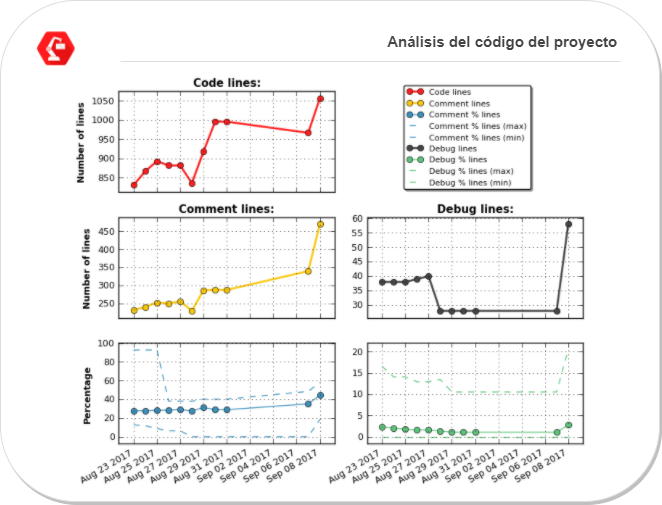
\includegraphics[width=0.75\textwidth]{figuras/SW/analisis_codigo.png}   
        \caption{Análisis del código del proyecto}
        \label{fig:SW:code_analysis}
    \end{figure}
    

 \chapter{Control} \label{chap:Control}
\hrule
\vspace{3mm}
En este capítulo se detalla el trabajo realizado dentro del ámbito de la ingeniería de control aplicada a este proyecto.

\section{Control de velocidad para los servos G15 cube} \label{sec:Control:velocidad_g15}

Los \glosarioPlural{servo} de Cytron aún teniendo diferentes modos de control no poseen un control efectivo de la velocidad de rotación cuando se utilizan en el modo de giro continuo o \ingles{wheel mode}.

 %\chapter{Cómo escribir en Latex}

\section{Citas}

%las referencias a artículos se ponen con \cite, 
%las referencias a imágenes \ref, 
%y las referencias a ecuaciones \eqref

Esto es un ejemplo de cita de un artículo \cite{Brunete:2013}.


\section{Listas}

%itemize es una lista. Cada término lleva delante un \item
Ejemplo de lista de puntos:
\begin{itemize}
\item Ejemplo1.
\item Ejemplo2.
\end{itemize} 

Y lista numerada:
\begin{enumerate}
\item Elemento 1
\item Elemento 2
\end{enumerate}

\section{Tablas}

Ejemplo de tabla. Como se aprecia en la tabla \ref{tab:table_example}...
\begin{table}[tb]
\caption{Ejemplo de tabla}
\label{tab:table_example}
\begin{center}
\begin{tabular}{|c||c|c|}
\hline
One & Two & Three\\
\hline
F1A & F1B & F1C\\
F2A & F2B & F2C\\
\hline
\end{tabular}
\end{center}
\end{table}

\section{Referencia a una sección}
\label{sec:refsec}

Ejemplo de referencia a la sección \ref{sec:refsec}

\section{Texto}

Testo en \textbf{negrita} y \textit{cursiva}.

\section{Figuras}

Ejemplo de referencia a figura (figura \ref{fig:logo_upm}). Es importante que todas las figuras que aparezcan están referenciadas, as� como las tablas. En general las figuras se colocarán al principio o al final de cada página ([tb] en latex), a no ser que por alguna necesidad se deban colocar en una posición exacta ([h]).

%caption es el pie de foto, y label es el nombre que se da a la imagen para referenciarla después. label no puede llevar acentos y no se muestra de cara al documento final (es sólo interno).
\begin{figure}[tb]
\centering

\includegraphics[width=0.45\textwidth]{figuras/Logo_UPM.jpg}   
\caption{Logotipo de la UPM}
\label{fig:logo_upm}
\end{figure}

 \chapter{Resultados y discusión} \label{chap:Resultados}
\chapterimage{figuras/ImagenesPortada/PortadaResultados.jpg}
\hrule
\vspace{3mm}

En este capítulo...


\section{Resultados}


\section{Discusión}


 \chapter{Gestión del proyecto} \label{chap:Gestion}
\chapterimage{figuras/ImagenesPortada/PortadaPlanificacion.jpg}
\hrule
\vspace{3mm}

En este capítulo se describe la gestión del proyecto: ciclo de vida, planificación, presupuesto, etc.

\section{Ciclo de vida}

Explicación de las fases del proyecto: definición, análisis, diseño, construcción, pruebas, implementación, validación, documentación. Ejemplo: diagrama de Pert.

\section{Planificación}

Se puede indicar mediante un diagrama de Gantt.

\subsection{Planificación inicial}

\subsection{Planificación final}


\section{Presupuesto}

    Coste de los materiales en la Tabla \ref{tab:presupuesto}:

    \completar

    \renewcommand{\thempfootnote}{\arabic{mpfootnote}}

    \begin{table}[H]
    \caption{Costes del proyecto}
    \label{tab:presupuesto}
    \begin{center}
    \begin{minipage}{\textwidth}
    \begin{tabular}{ |c|c|c|c| }
    \hline
    Artículo & Coste Unitario\footnote{En los casos en qué ha sido necesario se ha aplicado el cambio a Euros oficial propuesto por el Banco de España en el día en que se han consultado los precios: \url{https://www.bde.es/bde/es/}} & $N^o$ de unidades & Total\\
    \hline
    \hline
    Arduino Uno & 17.00 \euro\footnote{Precios consultados en la página oficial de Arduino a 07 de Septiembre 2017 (\url{https://store.arduino.cc/arduino-uno-rev3}).} & 1 & 17.00 \euro\\
    Cytron G15 Cube Servo & 23.23 \euro\footnote{Precios consultados en la página oficial de Cytron a 07 de Septiembre 2017 (\url{http://www.cytron.com.my/p-g15}).} & 3 & total\\
    Cytron G15 Shield & 6.64 \euro\footnote{Precio consultados en la página oficial de Cytron a 07 de Septiembre 2017 (\url{https://www.cytron.com.my/p-shield-g15}).} & 1 & 6.64 \euro\\
    \hline
    \hline
    Potenciómetro Serie TW & 9.29 \euro\footnote{Precio consultados en la página oficial de RS a 07 de Septiembre 2017 (\url{http://uk.rs-online.com/web/p/potentiometers/5028586/})} & 2 & 18.58\euro \\
    \hline
    \hline
    Barras Aluminio sección cuadrada & 5,626 \euro\footnote{Precio consultados en la página oficial de RS a 07 de Septiembre 2017 (\url{http://es.rs-online.com/web/p/tubos-de-aluminio/3047894/})} & 5 & 28,13 \euro \\
    Rodamiento 13x4 & 1.83\euro\footnote{Precio consultados en la página oficial de RS a 20 de Enero 2018 (\url{https://es.rs-online.com/web/p/rodamientos-de-bola/6189890/})} & & \euro \\
    Rodamiento 10x3 & 2.02\euro\footnote{Precio consultados en la página oficial de RS a 20 de Enero 2018 (\url{https://es.rs-online.com/web/p/rodamientos-de-bola/6189856/})} & & \euro \\
    Hilo Kevlar & 23.23 \euro\footnote{Precio consultados en la página de compra a 07 de Septiembre 2017 (\url{http://www.emmakites.com/index.php?main_page=product_info&cPath=336_365&products_id=1199})} & 1 & 23.23 \euro \\
    GM Series Plastic Wheel & 2.70 \euro\footnote{Precio consultados en la página oficial de Solarbotics a 11 de Septiembre 2017 (\url{https://solarbotics.com/product/gmpw/})} & 1 & 2.70 \euro \\
    \hline
    \end{tabular}
    \end{minipage}
    \end{center}
    \end{table}

    Poleas de acetal - https://es.rs-online.com/web/p/poleas-trapezoidales-con-perfil-en-v-de-transmision-mecanica/3520636/
     Soporte de sombrilla
\subsection{Personal}

\subsection{Material}

\subsection{Resumen de costes}


 \chapter{Conclusiones} \label{chap:Conclusiones}
\chapterimage{figuras/ImagenesPortada/PortadaConclusion.jpg}
\hrule
\vspace{3mm}

Se presentan a continuación las conclusiones...

\section{Conclusión} \label{sec:Conclusiones:Conclusion}

Una vez finalizado el proyecto...

\section{Desarrollos futuros} \label{sec:Conclusiones:Desarrollos_futuros}

Un posible desarrollo...


 \appendix
\addcontentsline{toc}{part}{\appendixname}

%\begin{appendices}

     \chapter{Listado de piezas diseñadas} \label{app:listadoPiezas}
         \hrule
         \vspace{3mm}
     	 \completar
\begin{center}
\begin{longtable}{|c|c|c|c|c|c|}
\caption{Listado de piezas diseñadas de fabricación propia}\\
\hline
\textbf{Num} & \textbf{Esquema Pieza} & \textbf{Referencia} & \textbf{Cantidad} & \textbf{Descripción} & \textbf{Peso Estimado}$^1$ \\
\hline
\endfirsthead
\multicolumn{5}{c}%
{\tablename\ \thetable\ -- \textit{Continuación de la página anterior}} \\
\hline
\textbf{Num} & \textbf{Esquema Pieza} & \textbf{Referencia} & \textbf{Cantidad} & \textbf{Descripción} & \textbf{Peso Estimado}$^1$ \\
\hline
\endhead
\multicolumn{5}{l}{\begin{minipage}{.8\linewidth}
	%do not draw the footnoterule
	\footnotesize{$^1$ El peso estimado se obtiene con el programa Cura \completar aplicando los parámetros de la tabla \ref{tab:listadoPiezas:param_impresion}. Este peso incluye el de los soportes necesarios para su impresión.}
\end{minipage}} \\ 
\hline \multicolumn{5}{r}{\textit{Continua en la página siguiente}} \\
\endfoot
\hline
%\insertTableNotes
\endlastfoot
1 & \iconoImagen{Base} & blah & 1  & blah & 193g \\
\hline
2 & \iconoImagen{RailA} & blah & 1 & blah & 24g \\
\hline
3 & \iconoImagen{RailB} & blah & 1 & blah & 24g \\
\hline
4 & \iconoImagen{PoleaMotor} & blah & 2 & blah & 3g \\
\hline
5 & \iconoImagen{EncajeTuboInterior} & blah & 1 & blah & 54g \\
\hline
6 & \iconoImagen{EncajeTuboExterior} & blah & 1 & blah & 128g \\
\hline
7 & \iconoImagen{FijacionBarraPieB} & blah & 1 & blah & blah \\
\hline
8 & \iconoImagen{FijacionBarraPie} & blah & 1 & blah & blah \\
\hline
10 & \iconoImagen{RuedaMotorGiroZ} & blah & 1 & blah & 18g \\
\hline
19 & \iconoImagen{AdaptadorPoleaNegra} & blah & 2 & blah & 1g \\
\hline
19 & \iconoImagen{AdaptadorPoleaNegra} & \completarCon{SeparadorPoleas} & 2 & blah & 20g \\
\hline
9 & \iconoImagen{SoportePlaca} & blah & 1 & 10g \\
\hline
11 & \iconoImagen{UnionBarrasIntermediasA} & blah & 1 & blah & blah \\
\hline
12 & \iconoImagen{UnionBarrasIntermediasB} & blah & 1 & blah & blah \\
\hline
13 & \iconoImagen{RuedaTransmisionSuperior} & blah & 1 & blah & 8g \\
\hline
14 & \iconoImagen{TapaPotenciometro} & blah & 1 & blah & blah \\
\hline
15 & \iconoImagen{EngranajePotenciometro} & blah & 1 & blah & blah \\
\hline
16 & \iconoImagen{EngranajeBarra} & blah & 1 & blah & blah \\
\hline
17 & \iconoImagen{UnionBarrasSuperiorA} & blah & 1 & blah & blah \\
\hline
18 & \iconoImagen{PoleaColumpioRedir} & blah & 3 & blah & blah \\
\hline
19 & \iconoImagen{CubrePoleaColumpio} & blah & 2 & blah & 6g \\
\hline
20 & \iconoImagen{CubrePoleaColumpioB} & blah & 2 & blah & blah \\
\hline
21 & \iconoImagen{CubrePoleaRedireccionB} & blah & 1 & blah & blah \\
\hline
22 & \iconoImagen{CubrePoleaRedireccion} & blah & 1 & blah & blah \\
\hline
23 & \iconoImagen{PiezaRodamientosSandwich} & blah & 2 & blah & 39g \\
\hline
24 & \iconoImagen{PiezaRodamientosSandwichB} & blah & 1 & blah & 39g \\
\hline
25 & \iconoImagen{PiezaRodamientosSandwichPotenciometro} & blah & 1 & blah & 44g \\
\hline 
26 & \iconoImagen{TapaPotenciometroA2} & blah & 1 & 1 & 2g \\
\hline
27 & \iconoImagen{PiezaMetacrilato} & blah & 2 & blah & - \\
\hline
28 & \iconoImagen{PiezaUnionSandwich} & blah & 4 & blah & 9g \\
\hline
29 & \iconoImagen{RealimentacionSandwich} & blah & 1 & blah & 24g \\
\hline
30 & \iconoImagen{SandwichAcoplamientoRodamientoBarra} & blah & 1 & blah & blah \\
\hline
\end{longtable}

\end{center}


\begin{center}
\begin{table}[H]
    \caption{Parámetros de las piezas para la estimación de peso}
    \label{tab:listadoPiezas:param_impresion}
    \begin{minipage}{\textwidth}
    \begin{tabular}{ |c|c|c|c| }
    \hline
    a & a & a & a \\ 
    %1 & \iconoImagen{Base}{0.2} & blah & \completar \\
    \hline
    \end{tabular}
    \end{minipage}
\end{table}
\end{center}

    	
     \chapter{Montaje del prototipo} \label{app:montajePiezas}
         \hrule
         \vspace{3mm}
%     	%\input{anexos/documentacionG15}
    	
     \chapter{Reglas de codificación del Software} \label{app:codificacionSW}
        \hrule
        \vspace{3mm}
     	Las reglas de codificación aplicadas al software del proyecto se han obtenido, por utilizar una referencia, de las reglas aplicadas por Google en sus proyectos libres. Esta guía está ampliamente documentada en \cite{googlecppguide} e incluye su propia herramienta para comprobar su correcta aplicación, Cpplint, lo que facilita la revisión del código así como corrección de desviaciones de estilo.
\\

En este anexo se traducen y resumen los aspectos más importantes de dicha guía. En algunos casos se han adaptado las reglas al caso concreto de este proyecto.
\\

Establecer unas reglas de codificación, unificando un estilo en la notación y uso de la sintaxis, es interesante de cara a posibilitar una mayor facilidad de lectura en futuros desarrollos aumentando así la mantenibilidad del código.

Estas reglas aplican al código C++ del proyecto, no a los \ingles{scripts} auxiliares.

\section{Aspectos generales} \label{sec:codificacionSW:general}

\section{Ficheros de cabecera} \label{sec:codificacionSW:cabeceras}

    En general todos los ficheros con extensión \codigo{.cpp} correspondientes a las librerías deberán ir acompañados del fichero de cabecera \codigo{.h} correspondiente.
    \\
    
    Quedan exentos de cumplir esta regla los ficheros correspondientes a Test (unitarios, de integración, etc) así como ficheros que contengan únicamente una función \codigo{main()}.

\minititulo{Inclusión Múltiple}

    Para evitar problemas de inclusión múltiple todos los ficheros de cabecera con extensión \codigo{.h} deberán incluir guardas con el siguiente formato y escrito en mayúsculas: \codigo{<nombre\_del\_fichero>\_<extensión>. } 
    \\ 
    
    \lstset{language=C, breaklines=true, basicstyle=\footnotesize}
    %Introducir label y caption
    \begin{lstlisting}[frame=single]
Ejemplo:

    #ifndef SERVO_RHA_H
    #define SERVO_RHA_H
    ...
    ...
    ...
    #endif
    \end{lstlisting}
    
\minititulo{Orden de inclusión de ficheros}

    Para evitar problemas en las dependencias de las distintas librerías se incluirán las mismas dejando para el final las librerías propias del proyecto e incluyendo el resto de la más general a la más particular. 
    \\ 
    
    \lstset{language=C, breaklines=true, basicstyle=\footnotesize}
    %Introducir label y caption
    \begin{lstlisting}[frame=single]
Ejemplo orden al incluir cabeceras:

    #include <stdint.h>    // lib estandar de c++
    #include <Arduino.h>     // lib de Arduino
    #include <SoftwareSerial.h>     // lib para controlar el puerto serie. Basado en Arduino
    
    #include "debug.h"     // def y control de las funciones de debug
    #include "rha_types.h"     // tipos de datos
    #include "joint_rha.h"     // clase a incluir
    \end{lstlisting}
    
    Nota: def. se utiliza de aquí en adelante como abreviatura de \ingles{definición}.
    
    Se deben incluir todos los ficheros que definan los símbolos utilizados en el fichero sobre el que se incluyen. Las declaraciones anticipadas de objetos no están permitidas salvo excepciones justificadas.
 
\section{Ámbitos}\label{sec:codificacionSW:ambitos}
\minititulo{Espacios de nombres}

    Como norma general las constantes, variables o funciones que no estén contenidas en ningún objeto se incluirán dentro de un espacio de nombres o \ingles{namespace} que haga referencia a la utilidad de las mismas.
    \\ 
    
    No está permitido usar directivas del tipo \codigo{ <using namespace \_\_\_\_;>.}
    \\ 
    
    Los espacios de nombres se escriben con la primera letra de cada palabra, en caso de haber más de una, en mayúscula y sin separación de ningún tipo.
    \\ 
    
    \lstset{language=C, breaklines=true, basicstyle=\footnotesize}
    %Introducir label y caption
    \begin{lstlisting}[frame=single]
Ejemplo: Constantes referentes al test de comportamiento ante una entrada tipo rampa

    namespace SlopeTest {
        #define SAMPLE_SLOPE 110
        #define SAMPLE_TEST_SLOPE 20
        #define SLOPE_SPEED 0.1
    }
    
Prohibido el uso de:
    
    using namespace StepTest;
    \end{lstlisting}
    
\minititulo{Variables Locales}

    Las variables se definirán preferiblemente en el ámbito más local en que se vayan a utilizar. Preferiblemente la inicialización de las mismas se hará junto a la declaración.
    \\ 
    
    Se pueden dar excepciones, como pueden ser vectores sobre los que se iterará dentro de un bucle u otros casos similares. En estos casos se de declarará el objeto fuera del propio ámbito para evitar recursivas llamadas a constructor y destructor de los mismos.
    \\ 
    
    \lstset{language=C, breaklines=true, basicstyle=\footnotesize}
    %Introducir label y caption
    \begin{lstlisting}[frame=single]
Ejemplo: 
    
    // Siempre que la variable sobre la que se itera no se vaya a utilizar para posteriores operaciones: 
    for(int i = 0, i < 10; i++) {
    }
    
    //mejor que el caso siguiente, que adicionalmente incumple la regla preferente de inicializar la variable cuando se declara:
    int i; 
    for(i = 0, i < 10; i++) {
    }
    
    //queda permitido declarar vectores u otros objetos similares antes si se va a iterar o trabajar sobre los mismos
    int vector[5] = {1,2,3,4,5};
    for(int i = 0, i < 10; i++) {
        Serial.print(vector[i]);
    }

    \end{lstlisting}
    
\section{Clases}\label{sec:codificacionSW:clases}

\minititulo{Constructores y métodos de Inicialización}

Para todos los objetos debe haber constructores por defecto sin parámetros de entrada. Aunque se pueden añadir constructores que inicialicen los diferentes parámetros será obligatorio generar métodos que los inicialicen una vez construido el objeto así como constructores por defecto para todos los métodos. Arduino, aún estando basado en el lenguaje \codigo{C++} no permite un uso completo de memoria dinámica. Los objetos se declaran como miembros haciendo uso del constructor por defecto para ser inicializados posteriormente.
\\ 

    \lstset{language=C, breaklines=true, basicstyle=\footnotesize}
    %Introducir label y caption
    \begin{lstlisting}[frame=single]
Ejemplo: 
    
	//NO se permite:
    - joint_rha.h -
    ServoRHA servo_*;
    - joint_rha.cpp -
    servo_ = new ServoRHA(1, 10, 5);
    
    //Se llama al constructor del objeto para luego inicializarlo:
    - joint_rha.h -
    ServoRHA servo_;
    - joint_rha.cpp -
    servo.init(... params ...);

    \end{lstlisting}

Para evitar funciones con muchos parámetros que reduzcan la legibilidad del código se permite generar diferentes inicializadores para los distintos parámetros. En la documentación del objeto deberá quedar bien claro que inicializadores deben invocarse para el correcto funcionamiento del mismo.

\minititulo{Estructuras o Clases}

Por norma general las estructuras se utilizarán exclusivamente para objetos pasivos, objetos que contienen información. Todo lo demás se codificará dentro una clase.
\\ 

En el caso de estructuras se permiten únicamente métodos para el manejo de los datos sin añadir ninguno tipo de comportamiento, están permitidos los constructores, destructores, métodos de reset, validación, etc. El acceso a los miembros de la estructura se hará directamente sobre los propios parámetros y no mediante métodos específicos. Los parámetros serán siempre públicos para ser consistente con este punto.
\\ 

Para mayores funcionalidades se generará una clase.

\minititulo{Control de Acceso}

Como norma general se declararan como privados todos los atributos de las clases exceptuando aquellos objetos que a su vez tengan, internamente, control de acceso definido (otras clases). De cara a generar Test con clases propias se permite la declaración de atributos como \codigo{protected}.

\section{Tipos de datos}\label{sec:codificacionSW:datos}

Los tipos de datos usados irán acordes con la librería \codigo{stdint.h}. Estos son del tipo \codigo{int16\_t}, \codigo{uint32\_t}, etc. Este tipo de datos garantiza el control del tamaño del dato declarado.

Se utilizarán los nombres \codigo{float} y \codigo{double} convencionales para declarar datos en coma flotante.

\section{Nombres}\label{sec:codificacionSW:nombres}

\minititulo{Reglas generales}

Los nombres deberán ser descriptivos. Por norma general no se utilizarán abreviaciones que no estén comúnmente aceptadas.

\minititulo{Nombre de los ficheros}

    Los nombres de los ficheros de código C++ se nombran en minúsculas separando, en caso de haber varias palabras, con un guión bajo. Los ficheros correspondientes a los test llevarán, precediendo al nombre la palabra "test".
    \\ 
    
    \lstset{language=C, breaklines=true, basicstyle=\footnotesize}
        %Introducir label y caption
        \begin{lstlisting}[frame=single]
Ejemplos:

    joint_handler.h
    joint_rha.cpp
    test_servo_rha.cpp
    \end{lstlisting}

\minititulo{Nombre de los directorios}

    Los ficheros de código irán contenidos en diferentes directorios para cada librería o conjunto de test. Estos directorios llevarán el nombre de la librería que contienen, en el mismo formato que la misma, en este caso sin extensión. Los test se ejecutan en el orden en que se ordenan los directorios. En este caso se añadirá un carácter para ordenar los mismos de manera adecuada. 
    \\ 
    
    Están exentos de esta regla los ficheros principales (que contienen la función \codigo{main()}, ó \codigo{setup()} y \codigo{loop()} en caso de ser ficheros con extensión \codigo{.ino}). 
    \\
    \lstset{language=C, breaklines=true, basicstyle=\footnotesize}
    %Introducir label y caption
    \begin{lstlisting}[frame=single]
Ejemplos:

/lib/
    joint_handler/
    joint_rha/
/test/
    a_test_servo_rha/
    b_test_joint_rha/
    \end{lstlisting}

\minititulo{Nombres para objetos}

Los nombres llevarán mayúscula al comienzo así como al inicio de cada palabra, sin guion bajo como separación.
\\ 

    \lstset{language=C, breaklines=true, basicstyle=\footnotesize}
    %Introducir label y caption
    \begin{lstlisting}[frame=single]
Ejemplo: 
    
    class ServoRHA{ ... };
    class JointHandler{ ... };
    struct SpeedGoal { ... } ;

    \end{lstlisting}
    
\minititulo{Nombres de variables}   

	Por norma general las variables se nombrarán en minúsculas, separando, cuando fuera necesario, las diferentes palabras mediante un guión bajo.
    
\minititulo{Nombres de atributos de clases}
   
La norma para nombrar atributos de clases será igual que en el caso general acabando, en este caso, con un guión bajo.
\\ 

    \lstset{language=C, breaklines=true, basicstyle=\footnotesize}
    %Introducir label y caption
    \begin{lstlisting}[frame=single]
Ejemplo: 
    
    class Regulator {
        float kp_, ki_, kd_;
        float ierror_[INTEGER_INTERVAL];
        uint8_t index_;    
    ... } ;

    \end{lstlisting}
    
\minititulo{Nombres de miembros de estructuras}
 
Las variables miembro de estructuras serán nombradas de igual forma que en el caso general.
\\ 

    \lstset{language=C, breaklines=true, basicstyle=\footnotesize}
    %Introducir label y caption
    \begin{lstlisting}[frame=single]
Ejemplo: 
    
    struct SpeedGoal {
        uint8_t servo_id;
        int16_t speed;
        int16_t speed_slope;
        uint8_t direction;  
    ... } ;

    \end{lstlisting}
    
\minititulo{Nombres de funciones} 

Las funciones comenzarán en minúscula marcando con mayúscula cada nueva palabra que aparezca. Los acrónimos irán en mayúscula. Esta regla afecta a métodos de clases a de igual manera a excepción de constructores y destructores.
\\ 

    \lstset{language=C, breaklines=true, basicstyle=\footnotesize}
    %Introducir label y caption
    \begin{lstlisting}[frame=single]
Ejemplo: 
    
  class ServoRHA {
 	...
 public:
    ServoRHA() { time_last_error_ = 0; time_last_ = 0; last_error_ = 0;
                error_ = 0; derror_ = 0; ierror_ = 0; }
    ServoRHA(uint8_t servo_id);
    void init(uint8_t servo_id);
    void addUpadteInfoToPacket(uint8_t *buffer);
    bool addTorqueToPacket(uint8_t *buffer);
    void setTorqueOnOfToPacket(uint8_t *buffer, uint8_t onOff);

  ... } ;

    \end{lstlisting}
    
\minititulo{Nombres de parámetros funciones} 
	
Los parámetros de métodos y funciones se nombran siguiendo el caso general para nombrar variables.
    
\minititulo{Espacios de nombres} 

Como se ha visto en la sección \ref{sec:codificacionSW:ambitos} los espacios de nombres se definen de manera equivalente a las clases. 

\minititulo{Nombres de enumeraciones} 

En el caso de enumeraciones se seguirá la misma norma que para las clases y espacios de nombres. En este caso cabe la excepción de poder ser declaradas sin nombre.

\minititulo{Nombres de macros} 

Todo nombre precedido por una instrucción \codigo{\#define} se nombrará en mayúsculas, separando las palabras, si las hubiera, mediante el uso del guión bajo. Esto aplica tanto a macros como constantes.

\section{Comentarios}\label{sec:codificacionSW:comentarios}

Es necesario el uso de comentarios para documentar el código y aumentar la legibilidad del mismo. En este caso se seguirá el estilo utilizado por \ingles{doxygen}, que será la herramienta utilizada para, posteriormente generar la documentación. 

\minititulo{Comentarios de ficheros}

Todos los ficheros deberán llevar comentarios en su cabecera. Estos comentarios tendrán el siguiente aspecto:
\\ 

    \lstset{language=C, breaklines=true, basicstyle=\footnotesize}
    %Introducir label y caption
    \begin{lstlisting}[frame=single]
Ejemplo: 
    
/**
 * @file
 * @brief Implements ServoRHA class. This object inherits from CytronG15Servo object to enhance its capabilities
 *
 * @Author: Enrique Heredia Aguado <enheragu>
 * @Date:   2017_Sep_08
 * @Project: RHA
 * @Filename: servo_rha.h
 * @Last modified by:   quique
 * @Last modified time: 30-Sep-2017
 */

    \end{lstlisting}


\minititulo{Comentarios de funciones}

Todas las funciones y métodos deberán llevar un comentario describiendo su funcionamiento así como los parámetros de entrada y salida. Estos comentarios tendrán el siguiente aspecto y se situarán encima de la definición de la función o método:
\\ 

    \lstset{language=C, breaklines=true, basicstyle=\footnotesize}
    %Introducir label y caption
    \begin{lstlisting}[frame=single]
Ejemplo: 
    
 /** @brief Saves in buffer the package return level of servo (error information for each command sent)
   * @method ServoRHA::addReturnOptionToPacket
   * @param {uint8_t*} buffer array in which add the information
   * @param {uint8_t} option RETURN_PACKET_ALL -> servo returns packet for all commands sent; RETURN_PACKET_NONE -> servo never retunrs state packet; RETURN_PACKET_READ_INSTRUCTIONS -> servo answer packet state when a READ command is sent (to read position, temperature, etc)
   * @see addToPacket()
   */

    \end{lstlisting}
    

\minititulo{Comentarios y aclaraciones}
	
    Cuando sea necesario hacer aclaraciones, a nivel de código se harán utilizando el estilo de comentario con doble barra \codigo{//}. Por lo general los nombres de variables y funciones deberán ser de por si descriptivas por lo que este tipo de comentarios se reservan para partes del código especialmente enrevesadas.
    \\ 
    Los comentarios, cuando vayan en línea con el código, se situarán a dos espacios del mismo, dejando un espacio entre el comentario en sí y la doble barra.
    
\minititulo{TODO y notas}

	En algunos casos se podrán dejar cosas para hacer en futuro (TODO) o notas aclaratorias (NOTE). En ambos casos se pondrá en mayúsculas y seguido de dos puntos. Quedando comentados mediante doble barra.
\\ 

    \lstset{language=C, breaklines=true, basicstyle=\footnotesize}
    %Introducir label y caption
    \begin{lstlisting}[frame=single]
Ejemplo: 

    // TODO: complete CW and CCW selection
    // NOTE: important the use of mascares to obtain direction os movement

    \end{lstlisting}
    
\minititulo{Código en desuso}

En algunas situaciones hay fragmentos de código que ya no se utilizan o están temporalmente deshabilitados. Estos fragmentos serán comentados mediante barra y asterisco :
\\ 

    \lstset{language=C, breaklines=true, basicstyle=\footnotesize}
    %Introducir label y caption
    \begin{lstlisting}[frame=single]
Ejemplo: 

	/* ... 
    ... some code ...
    ... */

    \end{lstlisting}
    
\section{Formato}\label{sec:codificacionSW:formato}

\minititulo{Espacios y tabulaciones}

Por norma general se utilizará cuatro espacios como indentación para distintos ámbitos. 
\\ 

    \lstset{language=C, breaklines=true, basicstyle=\footnotesize}
    %Introducir label y caption
    \begin{lstlisting}[frame=single]
Ejemplo: 

void ServoRHA::setWheelSpeedToPacket( ... ) {
    ...    
    if ( ... ) {
        ...
    }
    ...  
}

    \end{lstlisting}
    
\minititulo{Declaración y definición de funciones}

El valor de retorno así como los parámetros de una función deberán ir en la misma línea. En caso de no caber o para mayor claridad se pondrán a la misma altura que los anteriores.
\\ 

    \lstset{language=C, breaklines=true, basicstyle=\footnotesize}
    %Introducir label y caption
    \begin{lstlisting}[frame=single]
Ejemplo: 

    void ServoRHA::setWheelSpeedToPacket(uint8_t *buffer, uint16_t speed, uint8_t direction) {
	...
    }

    void ServoRHA::setWheelSpeedToPacket(uint8_t *buffer, uint16_t speed,
                                         uint8_t direction) {
	...
    }

    \end{lstlisting}
    
    
\minititulo{Condicionales}

Como norma general no se dejarán espacios entre los paréntesis. Si se dejará un espacio entre la sentencia \codigo{if} y el condicional, así como entre este último y la llave que abre el ámbito condicional.
\\ 

    \lstset{language=C, breaklines=true, basicstyle=\footnotesize}
    %Introducir label y caption
    \begin{lstlisting}[frame=single]
Ejemplo: 
//Forma correcta:
    if (direction == CW) {
        speed = speed | 0x0400;
    }
    
//Ejemplos incorrectos:
    if(direction == CW) {  // Falta un espacio tras la sentencia if
    if (direction == CW){  // Falta un espacio entre el condicional y la llave
    if(direction == CW){  // Combina los casos anteriores 

    \end{lstlisting}
    
    En caso de que el condicional afecte solo a una sentencia esta se pondrá, como norma general, sin llaves y en la misma línea que el condicional. De igual forma se hará tras sentencias de tipo \codigo{else} o combinando \codigo{else if}. En caso de utilizar llaves se seguirá la norma que aplica a dicho caso.
\\ 

    \lstset{language=C, breaklines=true, basicstyle=\footnotesize}
    %Introducir label y caption
    \begin{lstlisting}[frame=single]
Ejemplo: 

    if (speed1 < speed2-speed_margin) return ServoRHAConstants::LESS_THAN;
    else if (speed1 > speed2+speed_margin) return ServoRHAConstants::GREATER_THAN;
    else return ServoRHAConstants::EQUAL;

    \end{lstlisting}
    
    Cuando si afecta a diferentes líneas y hay sentencias de tipo \codigo{else}, estas irán en la misma línea de cierre de llave del condicional (siempre que no afecte a la legibilidad del código ya sea por presencia de comentarios u otras causas similares).
    \\ 

    \lstset{language=C, breaklines=true, basicstyle=\footnotesize}
    %Introducir label y caption
    \begin{lstlisting}[frame=single]
Ejemplo: 

    if (...) {
            ...
        } else {
            ...
        }

    \end{lstlisting}
    
\minititulo{Bucles}

El formato será equivalente al caso de los condicionales:
\\ 

    \lstset{language=C, breaklines=true, basicstyle=\footnotesize}
    %Introducir label y caption
    \begin{lstlisting}[frame=single]
Ejemplo: 

    for (...) {
       ...
    }
    for (...) oneLineStatement;
    while (condition) {
        ...
    }

    \end{lstlisting}  
    
    
\minititulo{Valor de retorno de funciones y métodos}

No es necesario utilizar paréntesis para rodear la expresión a retornar. Solo se utilizarán en los casos en que se utilizarían si se fuera a asignar dicha expresión a una variable.

\minititulo{Formato para clases}

Las directivas \codigo{public}, \codigo{protected} y \codigo{private} irán indentados un espacio respecto a la definición de la clase. Por norma general irán precedidos por una línea en blanco (excepto cuando las preceda la definición de la propia clase).
\\ 

    \lstset{language=C, breaklines=true, basicstyle=\footnotesize}
    %Introducir label y caption
    \begin{lstlisting}[frame=single]
Ejemplo: 


class JointHandler {
 private:  // un espacio
    ...
 public:
    ...

    \end{lstlisting} 
    
\minititulo{Espacios de nombre}

Los espacios de nombres siguen la norma general para indentar diferentes ámbitos.

\section{Espacios en blanco}\label{sec:codificacionSW:espacios_blanco}

Los espacios horizontales dependerán de cada caso. En ningún caso se finalizará una línea con un espacio en blanco.

\minititulo{Caso general}

    \lstset{language=C, breaklines=true, basicstyle=\footnotesize}
    %Introducir label y caption
    \begin{lstlisting}[frame=single]
Ejemplo: 

    void JointHandler::setTimer(uint64_t timer) {  // Un espacio entre el cierre del parentesis y la apertura de llaves
    class TimerMicroseconds : public Timer {  // Espacio entre los dos puntos en casos de herencia o inicializadores dentro de constructores. Se pone un espacio a cada lado.
    void checkWait()  // No se deja espacio entre el nombre y los parentesis. Tampoco entre parentesis vacios.
    float getError() { return error_; }  // Se deja espacio entre llaves e implementacion, a ambos lados.

    \end{lstlisting}

\minititulo{Bucles, condicionales y estructuras de control}

    \lstset{language=C, breaklines=true, basicstyle=\footnotesize}
    %Introducir label y caption
    \begin{lstlisting}[frame=single]
Ejemplo: 

    if (b) {  // Espacio entre la sentencia if y la condicion, asi como esta misma con la apertura de llaves
    } else {  // Espacios al rededor de la sentencia else
    }
    switch (i) {
        case 1:  // No se deja espacio antes de los dos puntos
        ...
        case 2: break;  // Si se deja despues de los mismos
    for (int i = 0 ; i < 5 ; i++) {  // En caso de bucles for, ademas de los espacios al rededor de los parentesis se dejara un espacio tras cada punto y coma.
    \end{lstlisting}
    
\minititulo{Operadores}

    \lstset{language=C, breaklines=true, basicstyle=\footnotesize}
    %Introducir label y caption
    \begin{lstlisting}[frame=single]
Ejemplo: 

    // En general se deja un espacio al rededor de los distintos tipos de operadores
    x = 0;
    v = w * x + y / z;
    v = w*x + y/z;
    v = w * (x + z);
    
    // No se separan operadores unarios de sus argumentos:
    x = -5;
    x++;
    if (x && !y)

    \end{lstlisting}
    

\section{Espacio vertical}

Por lo general se dejaran espacios verticales para una mayor claridad del código sin abusar de los mismos. Aunque separar diferentes partes puede ayudar demasiados espacios verticales pueden dificultar la lectura de código.

    
     \chapter{Documentación del software} \label{app:documentacion_software}
         \hrule
         \vspace{3mm}
     	 %\include{doxygen_documentation/refman}
%\input{doxygen_documentation/refman}


     	 
     \chapter{Registros Servos G15} \label{app:registros_g15}
	     \hrule
	     \vspace{3mm}
	         En este anexo se describe como se trabaja con el protocolo de comunicación a bajo nivel para codificar el paso de mensajes entre los servos G15 Cube y el microcontrolador. 
    \\
    
    Antes de describir el formato de la información cabe destacar que en todo momento la información enviada irá codificada en formato hexadecimal, para los paquetes enviados como recibidos desde el microcontrolador. Todos los paquetes, tanto los enviados a los servos como la respuesta por parte de los mismos tendrán en común la siguiente información:
    
    \begin{itemize}
    	\item Encabezado: Los primeros dos bytes del mensaje estarán compuestos por encabezado que será el que marque el inicio del mensaje. Estos bytes serán: 0xFF 0xFF
    	\item Un fin de mensaje: El último byte del mensaje estará marcado por un valor llamado \ingles{CheckSum} que será el encargado de verificar que todo el paquete ha llegado correctamente. El \ingles{CheckSum} es el inverso del valor binario de la suma de todos los bytes enviados a excepción del encabezado y el propio \ingles{CheckSum}. En la figura \completar se puede ver un ejemplo de como se calcula dicho valor.
    \end{itemize}
    
    \completarCon{Ejemplo de como se calcula el checksum}
    
    En los paquetes que se envíen a los servos la información se codificará de la siguiente manera concreta:
    
    \begin{itemize}
    	\item Bytes 0 y 1: reservados para el encabezado.
    	\item Byte 2: codifica el ID del servo al que se quiere enviar la acción. De forma general se puede utilizar la dirección 0xFE (en hexadecimal) para enviar el mensaje a todos los servos conectados.
    	\item Byte 3: codifica la longitud del mensaje. Contando a partir del encabezado y el ID (excluyendo ambos) el número de bytes que se envían. De esta forma, al recibirse el paquete se podrá identificar el inicio del mismo, a que servo va dirigido (el resto ignorarán el paquete) y cuantos bytes tendrá que leer el aludido. Por supuesto el último byte de la cadena será el ya mencionado \ingles{CheckSum} cuyo valor tendrá que coincidir con el esperado al analizar la cadena.
    	\item Byte 4: codifica la instrucción que se desea realizar. Sobre la memoria de los servos se podrán hacer operaciones de lectura y escritura de distinta manera. Se pueden ver las diferentes instrucciones posibles en la tabla \ref{tab:g15_instructions}. Serán explicadas posteriormente más en detalle.
    	\item Bytes del 5 al N: Parámetros que se quieran enviar al servo.
    	\item Byte N+1: \ingles{CheckSum}
    \end{itemize}
    
    En la figura \ref{fig:app:registrosg15:comunicacion_mensaje} se puede ver representado, a modo de resumen gráfico, este esquema de información genérico.	
    
    \begin{figure}[H]
    	\centering
    	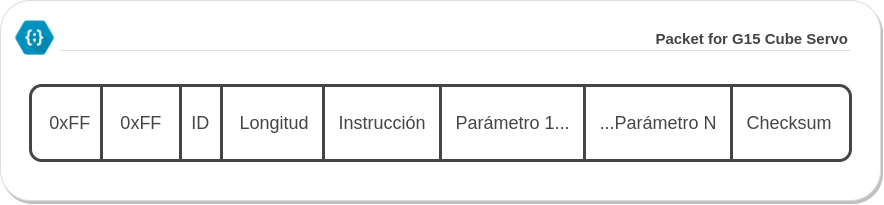
\includegraphics[width=0.9\textwidth]{figuras/Imagenes_SW/Packet_G15.png}   
    	\caption{Paquete de información genérico para comunicar con los Servos G15 Cube}
    	\label{fig:app:registrosg15:comunicacion_mensaje}
    \end{figure}
	

	\begin{table}[htbp]
		\centering
		\caption{Resumen de las instrucciones aceptadas por los Cytron G15 Cube servo}
		\label{tab:g15_instructions}
		\begin{center}
			\begin{tabular}{|c|c|c|}
			\hline
			\textbf{Instrucción} & \textbf{Valor Hex.} & \textbf{Comentarios} \\
			\hline
			iPING & 0x01 & Solicita un paquete con el estado del servo \\
			\hline
			iREAD\_DATA & 0x02 & Lee información de la memoria del servo \\
			\hline
			iWRITE\_DATA & 0x03 & Escribe información en la memoria del servo \\
			\hline
			iREG\_WRITE & 0x04 & Escribe sobre la memoria y hasta que llega la acción \ingles{ACTION} para ejecutar dichos cambios \\
			\hline
			iACTION & 0x05 & Activa la acción codificada con la instrucción \ingles{REG\_WRITE} \\
			\hline
			iRESET & 0x06 & Resetea la memoria a los valores por defecto \\
			\hline
			iSYNC\_WRITE & 0x83 & Para escribir simultáneamente información sobre varios servos \\
			\hline
			\end{tabular}
		\end{center}
	\end{table}	
	
	La respuesta por parte de los servos tiene también una estructura general que se detalla a continuación byte a byte:
	\begin{itemize}
		\item Bytes 0 y 1 de encabezado. Igual que en el caso anterior.
		\item Byte 2: codifica el ID del servo que responde.
		\item Byte 3: codifica la longitud a leer.
		\item Byte 4: sirve para informar de posibles errores en el servo. Cada bit del byte codifica un tipo de error, estando todos a 0 cuando la comunicación y el servo se encuentran buen estado. Estos errores están detallados en la tabla \ref{tab:g15_error}, junto a la máscara en binario que se aplicará a dicho byte para comprobar cada error.
		\item Bytes del 5 al N: Parámetros que envía el servo.
		\item Byte N+1: \ingles{CheckSum}.
	\end{itemize}
	
	 En la figura \ref{fig:app:registrosg15:comunicacion_mensaje_from_servo} se puede ver representado, a modo de resumen gráfico, este esquema de información genérico que se ha expuesto previamente.	
	 
	 \begin{figure}[H]
	    	\centering
	    	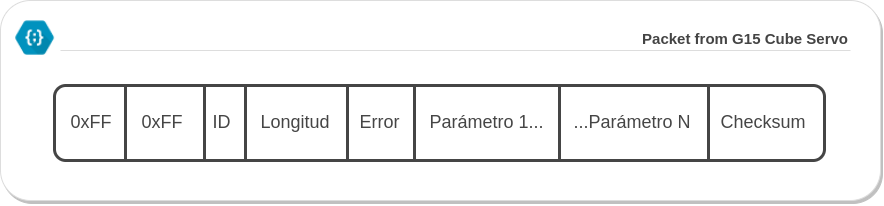
\includegraphics[width=0.9\textwidth]{figuras/Imagenes_SW/Packet_From_G15.png}   
	    	\caption{Paquete de información genérico de retorno de los Servos G15 Cube}
	    	\label{fig:app:registrosg15:comunicacion_mensaje_from_servo}
	 \end{figure}
	
	\begin{table}[htbp]
		\centering
		\caption{Codificación del error de los servos G15 Cube en cada bit del byte de error.}
		\label{tab:g15_error}
		\begin{center}
			\begin{tabular}{|c|c|c|}
				\hline
				\textbf{Bit} & \textbf{Error} & \textbf{Máscara a aplicar} \\
				\hline
				0 & Error en voltaje de entrada & 0X0001 \\
				\hline
				1 & Límite de ángulo & 0X0002 \\
				\hline
				2 & Sobrecalentamiento & 0X0004 \\
				\hline
				3 & Error en el rango pedido & 0X0008 \\
				\hline
				4 & Error en el \ingles{CheckSum} & 0X0010 \\
				\hline
				5 & Sobrecarga & 0X0020 \\
				\hline
				6 & Instrucción incorrecta & 0X0040 \\
				\hline
				7 & - & -  \\
				\hline
			\end{tabular}
		\end{center}
	\end{table}
	
	Aunque como se ha visto anteriormente y se ha detallado en la tabla \ref{tab:g15_error} el servo devuelve un solo byte de error, al leer la información recibida el error, tanto en la librería de Cytron como en la estructura desarrollada para este proyecto este byte se amplia a dos bytes para añadir la posibilidad de nuevos errores en la recepción del paquete de datos. Se pueden ver de forma detallada en la tabla \ref{tab:g15_error_second}, nuevamente junto a la máscara que se aplicará a dicho byte para cada caso. En el byte más bajo queda la información que devuelve el servo y en el más alto la información añadida.
	\\ 
	
	\begin{table}[htbp]
		\centering
		\caption{Codificación del error de comunicación en cada bit del segundo byte de error.}
		\label{tab:g15_error_second}
		\begin{center}
			\begin{tabular}{|c|c|c|}
				\hline
				\textbf{Bit} & \textbf{Error} & \textbf{Máscara a aplicar} \\
				\hline
				8 & Paquete perdido o tiempo de espera superado & 0X0100 \\
				\hline
				9 & Encabezado incorrecto & 0X0200 \\
				\hline
				10 & ID incorrecto & 0X0400 \\
				\hline
				11 & Error en el \ingles{CheckSum} & 0X0800 \\
				\hline
				12 & - & -  \\
				\hline
				13 & - & -  \\
				\hline
				14 & - & -  \\
				\hline
				15 & - & -  \\
				\hline
			\end{tabular}
		\end{center}
	\end{table}
	\section{Distintos tipos de instrucciones}
	A continuación se detallan las distintas instrucciones que aceptan los Servos, presentadas en la tabla \ref{tab:g15_instructions}.
	\subsection{Petición del estado del servo}
	
	Se hace una petición del estado o una operación de tipo \ingles{PING} cuando se quiere conocer la existencia y estado de un servo con un ID específico. Adicionalmente si se envía utilizando el ID comodín (0xFE, para todos los servos) se podrá recoger el ID del servo conectado (cuando solo haya uno).
	\\ 
	
	Un paquete para una operación \ingles{PING} podría tener el siguiente aspecto (\ingles{iPING} al servo con ID 1. El mensaje enviado tendrá una longitud de dos bytes a leer. Las diferentes instrucciones se han visto en la tabla \ref{tab:g15_instructions}):
	\begin{center}
		\begin{tabular}{|c|c|c|c|c|c|}
			\hline
			0xFF & 0xFF & 0x01 & 0x02 & 0x01 & 0xFB \\
			\hline
		\end{tabular}
	\end{center}
	
	Como se puede ver este mensaje no lleva parámetros.
	\\ 
	
	El mensaje de retorno podría ser, por ejemplo el siguiente. Respondiendo el servo con ID 1 dos bytes a leer, el error que es 0 (todo correcto) y el \ingles{CheckSum}:
	\begin{center}
		\begin{tabular}{|c|c|c|c|c|c|}
			\hline
			0xFF & 0xFF & 0x01 & 0x02 & 0x00 & 0xFC \\
			\hline
		\end{tabular}
	\end{center}
	
	\subsection{Operaciones de lectura} 
	
	Las operaciones de lectura, con la instrucción \ingles{iREAD\_DATA} vista en la tabla \ref{tab:g15_instructions} están pensadas para leer la memoria interna de los servos. Los parámetros enviados serán la dirección de memoria a partir de la cual se quiere leer y el número de bytes a leer. Se puede ver en la tabla \ref{tab:g15_register} las posibles direcciones de memoria a las que acceder, el tipo de acceso que tienen (lectura/escritura o ambos) así como los valores típicos (por defecto, máximos y mínimos).
	\\ 
	
	Un ejemplo de este tipo de mensajes puede ser una petición de lectura de la temperatura (0x2B en la tabla \ref{tab:g15_register}). En este caso sobre el servo con ID 1. La temperatura ocupa un solo byte.
		
	\begin{center}
		\begin{tabular}{|c|c|c|c|c|c|c|c|}
			\hline
			0xFF & 0xFF & 0x01 & 0x04 & 0x02 & 0x2B & 0x01 & 0xCC \\
			\hline
		\end{tabular}
	\end{center}
	
	Como en el caso anterior el paquete de retorno devolverá el ID del servo que responde, la longitud, que en este caso será de 3 bytes, y el error, el parámetro leido (un byte con la temperatura) y el \ingles{CheckSum}:
	
	\begin{center}
		\begin{tabular}{|c|c|c|c|c|c|c|}
			\hline
			0xFF & 0xFF & 0x01 & 0x03 & 0x00 & 0x20 & 0xDB \\
			\hline
		\end{tabular}
	\end{center}
	
	\subsection{Operaciones de escritura} \label{subsec:registros:operaciones:escritura}
	
	Las operaciones de escritura tienen un funcionamiento análogo al de lectura. La instrucción \ingles{iWRITE\_DATA} vista en la tabla \ref{tab:g15_instructions} envía una cadena de bytes a escribir a partir de una dirección de memoria dada. Nuevamente se pueden ver las direcciones de memoria en la tabla \ref{tab:g15_register}.
	\\ 
	
	Como ejemplo se escribirá, sobre el servo con ID 1 un ángulo objetivo (empieza en la dirección 0x1E). Como se puede ver ocupa dos bytes, empezando por el de más bajo y a continuación el más alto. A la hora de enviar el mensaje hay que tener en cuenta estos aspectos para que los parámetros vayan ordenados de igual manera:
	
	\begin{center}
		\begin{tabular}{|c|c|c|c|c|c|c|c|c|}
			\hline
			0xFF & 0xFF & 0x01 & 0x05 & 0x03 & 0x1E & 0xAA & 0x00 &0x2E  \\
			\hline
		\end{tabular}
	\end{center}
	
	El paquete de retorno en este caso devolverá el posible error en la comunicación, sin parámetros.
	\begin{center}
		\begin{tabular}{|c|c|c|c|c|c|}
			\hline
			0xFF & 0xFF & 0x01 & 0x02 & 0x00 & 0xFC \\
			\hline
		\end{tabular}
	\end{center}
	
	\subsection{Operaciones de escritura con activación desacoplada}
		
		La idea de este tipo de operación es la de enviar a distintos servos operaciones de escritura pero que queden pendientes de ejecutarse. De esta forma, utilizando la instrucció \ingles{iACTION} se podrán activar todos a la vez.
		\\ 
		
		Para la operación de escritura en memoria se seguirá un formáto análogo al descrito en el apartado \ref{subsec:registros:operaciones:escritura}. El único cambio es que la instrucción utilizada, en vez de ser \ingles{iWRITE\_DATA} como se ha descrito en dicho apartado, se utilizará la instrucción \ingles{iREG\_WRITE} (se puede consultar en la tabla \ref{tab:g15_instructions}).
		\\ 
		
		Una vez enviada la información a escribir a todos los servos, se procederá a enviar el mensaje de activación. En este caso se enviará a todos los servos conectados (ID genérico de 0xFE):
		\begin{center}
			\begin{tabular}{|c|c|c|c|c|c|}
				\hline
				0xFF & 0xFF & 0xFE & 0x02 & 0x05 & 0xFA \\
				\hline
			\end{tabular}
		\end{center}
		
		Por norma general, en los casos en los que se utiliza el ID genérico (menos en el caso de la instrucción \ingles{iPING} en los que hay un servo conectado) no se recogerá mensaje de retorno alguno.
		
	\subsection{Resetear la memoria de los servos a los valores de fábrica}
	
		La instrucción \ingles{iRESET} devolverá la memoria al estado por defecto. Se pueden ver los valores por defecto en la tabla \ref{tab:g15_register}.
		\\
		
		Para efectuarla se enviará dicha instrucción al servo correspondiente, en este caso al servo cuyo ID es 0:
		\begin{center}
			\begin{tabular}{|c|c|c|c|c|c|}
				\hline
				0xFF & 0xFF & 0x00 & 0x02 & 0x06 & 0xF7 \\
				\hline
			\end{tabular}
		\end{center}
		
		 Nuevamente el mensaje de error contendrá unicamente el posible error en la comunicación.
		 \begin{center}
		 	\begin{tabular}{|c|c|c|c|c|c|}
		 		\hline
		 		0xFF & 0xFF & 0x00 & 0x02 & 0x00 & 0xFD \\
		 		\hline
		 	\end{tabular}
		 \end{center}
		 
		 Se debe tener en cuenta, que aunque el mensaje de retorno responda con el valor inicial, una vez ejecutado el reset de la memoria el ID del servo valdrá 1 y el \ingles{baud rate} será de $19.2kb/s$
	
	\subsection{Operaciones de escritura sobre múltiples servos}
	
	\subsection{Aspectos interesantes a tener en cuenta}
		\completarCon{Cambiar de wheel mode a no wheel mode, control de velocidad que es falso, es torque lo que se pasa en wheel mode...
		¿Leer el torque que significa?}

\begin{table}[htbp]
	\caption{Características mas importantes de los Servos G15 de Cytron. Tabla traducida y resumida a los puntos más importantes del Cytron G15 Cube servo User Manual \cite{CytronTechnologies2012} \completarCon{¿esto está bien, hay que poner paginas involucradas?}}
	\label{tab:g15_register}
	\begin{adjustwidth}{-1.9cm}{-1.5cm}
	\begin{tabular}{|c|c|c|c|c|c|c|}
		\hline
		\textbf{Area} & \textbf{\shortstack{Address\\ (Hex)}} & \textbf{Parameter} & \textbf{\shortstack{Read only \\ /Read Write}} & \textbf{\shortstack{Factory\\ default\\ value (Hex)}} & \textbf{\shortstack{Minimum\\ value (Hex)}} & \textbf{\shortstack{Maximum\\ value (Hex)}} \\ \hline
		\multicolumn{ 1}{|c|}{EEPROM} & 0 (0x00) & Model (L) & R & ‘G’ (0x0F) & - & - \\ \cline{ 2- 7}
		\multicolumn{ 1}{|c|}{} & 1 (0x01) & Model(H) & R & 15 (0x47) & - & - \\ \cline{ 2- 7}
		\multicolumn{ 1}{|c|}{} & 2 (0x02) & Firmware Revision & R &  & - & - \\ \cline{ 2- 7}
		\multicolumn{ 1}{|c|}{} & 3 (0x03) & ID & RW & 1 (0x01) & 0 (0x00) & 253 (0xFD) \\ \cline{ 2- 7}
		\multicolumn{ 1}{|c|}{} & 4 (0x04) & Baud Rate & RW & 103 (0x67) & 3 (0x03) & 255 (0xFF) \\ \cline{ 2- 7}
		\multicolumn{ 1}{|c|}{} & 5 (0x05) & Return Delay & RW & 250 (0xFA)  & 1 (0x01)  & 255 (0xFF) \\ \cline{ 2- 7}
		\multicolumn{ 1}{|c|}{} & 6 (0x06) & CW Angle Limit (L) & RW & \multicolumn{ 1}{c|}{ 0 (0x0000) } & \multicolumn{ 1}{c|}{ 0 (0x0000) } & \multicolumn{ 1}{c|}{1087 (0x043F)} \\ \cline{ 2- 4}
		\multicolumn{ 1}{|c|}{} & 7 (0x07) & CW Angle Limit (H) & RW & \multicolumn{ 1}{c|}{} & \multicolumn{ 1}{c|}{} & \multicolumn{ 1}{c|}{} \\ \cline{ 2- 7}
		\multicolumn{ 1}{|c|}{} & 8 (0x08) & CCW Angle Limit (L) & RW & \multicolumn{ 1}{c|}{1087 (0x043F)} & \multicolumn{ 1}{c|}{ 0 (0x0000) } & \multicolumn{ 1}{c|}{1087 (0x043F)} \\ \cline{ 2- 4}
		\multicolumn{ 1}{|c|}{} & 9 (0x09) & CCW Angle Limit (H) & RW & \multicolumn{ 1}{c|}{} & \multicolumn{ 1}{c|}{} & \multicolumn{ 1}{c|}{} \\ \cline{ 2- 7}
		\multicolumn{ 1}{|c|}{} & 10 (0x0A) & Reserved & - & - & - & - \\ \cline{ 2- 7}
		\multicolumn{ 1}{|c|}{} & 11 (0x0B) & Temperature Limit & RW & 70 (0x46) & 0 (0x00) &  \\ \cline{ 2- 7}
		\multicolumn{ 1}{|c|}{} & 12 (0x0C) & Lowest Voltage Limit & RW & 65 (0x41) & 65 (0x41) & 178 (0xB2) \\ \cline{ 2- 7}
		\multicolumn{ 1}{|c|}{} & 13 (0x0D) & Highest Voltage Limit & RW & 150 (0x96)  &  &  \\ \cline{ 2- 7}
		\multicolumn{ 1}{|c|}{} & 14 (0x0E) & Max Torque (L) & RW & \multicolumn{ 1}{c|}{1023 (0x03FF)} & \multicolumn{ 1}{c|}{ 0 (0x0000) } & \multicolumn{ 1}{c|}{1023 (0x03FF)} \\ \cline{ 2- 4}
		\multicolumn{ 1}{|c|}{} & 15 (0x0F) & Max Torque (H) & RW & \multicolumn{ 1}{c|}{} & \multicolumn{ 1}{c|}{} & \multicolumn{ 1}{c|}{} \\ \cline{ 2- 7}
		\multicolumn{ 1}{|c|}{} & 16 (0x10) & Return Packet Enable & RW & 2 (0x02) & 0 (0x00) & 2 (0x02) \\ \cline{ 2- 7}
		\multicolumn{ 1}{|c|}{} & 17 (0x11) & Alarm LED & RW & 36 (0x24) & 0 (0x00) & 127 (0x7F) \\ \cline{ 2- 7}
		\multicolumn{ 1}{|c|}{} & 18 (0x12) & Alarm Shutdown & RW & 36 (0x24) & 0 (0x00) & 127 (0x7F) \\ \cline{ 2- 7}
		\multicolumn{ 1}{|c|}{} & 19 (0x13) & Reserved & - & - & - & - \\ \cline{ 2- 7}
		\multicolumn{ 1}{|c|}{} & 20 (0x14) & Down Calibration (L) & R &  &  &  \\ \cline{ 2- 7}
		\multicolumn{ 1}{|c|}{} & 21 (0x15) & Down Calibration (H) & R &  &  &  \\ \cline{ 2- 7}
		\multicolumn{ 1}{|c|}{} & 22 (0x16) & Up Calibration (L) & R &  &  &  \\ \cline{ 2- 7}
		\multicolumn{ 1}{|c|}{} & 23 (0x17) & Up Calibration (H) & R &  &  &  \\ \hline
		\multicolumn{ 1}{|c|}{RAM} & 24 (0x18) & Torque Enable & RW & 0 (0x00) & 0 (0x00) & 1 (0x01) \\ \cline{ 2- 7}
		\multicolumn{ 1}{|c|}{} & 25 (0x19) & LED & RW & 0 (0x00) & 0 (0x00) & 1 (0x01) \\ \cline{ 2- 7}
		\multicolumn{ 1}{|c|}{} & 26 (0x1A) & CW Compliance Margin & RW & 1 (0x01) & 0 (0x00) & 254(0xFE) \\ \cline{ 2- 7}
		\multicolumn{ 1}{|c|}{} & 27 (0x1B) & CCW Compliance & RW & 1 (0x01) & 0 (0x00) & 254(0xFE) \\ \cline{ 2- 7}
		\multicolumn{ 1}{|c|}{} & 28 (0x1C) & CW Compliance Slope & RW & 32 (0x0020) & 1 (0x01) & 254(0xFE) \\ \cline{ 2- 7}
		\multicolumn{ 1}{|c|}{} & 29 (0x1D) & CCW Compliance Slope & RW & 32 (0x0020) & 1 (0x01) & 254(0xFE) \\ \cline{ 2- 7}
		\multicolumn{ 1}{|c|}{} & 30 (0x1E) & Goal Position (L) & RW & Address 36 & \multicolumn{ 1}{c|}{ 0 (0x0000) } & \multicolumn{ 1}{c|}{1087 (0x043F)} \\ \cline{ 2- 5}
		\multicolumn{ 1}{|c|}{} & 31 (0x1F) & Goal Position (H) & RW & Address 37 & \multicolumn{ 1}{c|}{} & \multicolumn{ 1}{c|}{} \\ \cline{ 2- 7}
		\multicolumn{ 1}{|c|}{} & 32 (0x020) & Moving Speed (L) & RW & \multicolumn{ 1}{c|}{ 0 (0x0000) } & \multicolumn{ 1}{c|}{ 0 (0x0000) } & \multicolumn{ 1}{c|}{1023 (0x03FF)} \\ \cline{ 2- 4}
		\multicolumn{ 1}{|c|}{} & 33 (0x21) & Moving Speed (H) & RW & \multicolumn{ 1}{c|}{} & \multicolumn{ 1}{c|}{} & \multicolumn{ 1}{c|}{} \\ \cline{ 2- 7}
		\multicolumn{ 1}{|c|}{} & 34 (0x22) & Torque Limit (L) & RW & Address 14 & \multicolumn{ 1}{c|}{ 0 (0x0000) } & \multicolumn{ 1}{c|}{1023 (0x03FF)} \\ \cline{ 2- 5}
		\multicolumn{ 1}{|c|}{} & 35 (0x23) & Torque Limit (H) & RW & Address 15 & \multicolumn{ 1}{c|}{} & \multicolumn{ 1}{c|}{} \\ \cline{ 2- 7}
		\multicolumn{ 1}{|c|}{} & 36 (0x24) & Present Position (L) & R & \multicolumn{ 1}{c|}{} & \multicolumn{ 1}{c|}{} & \multicolumn{ 1}{c|}{} \\ \cline{ 2- 4}
		\multicolumn{ 1}{|c|}{} & 37 (0x25) & Present Position (H) & R & \multicolumn{ 1}{c|}{} & \multicolumn{ 1}{c|}{} & \multicolumn{ 1}{c|}{} \\ \cline{ 2- 7}
		\multicolumn{ 1}{|c|}{} & 38 (0x26) & Present Speed (L) & R & \multicolumn{ 1}{c|}{} & \multicolumn{ 1}{c|}{} & \multicolumn{ 1}{c|}{} \\ \cline{ 2- 4}
		\multicolumn{ 1}{|c|}{} & 39 (0x27) & Present Speed (H) & R & \multicolumn{ 1}{c|}{} & \multicolumn{ 1}{c|}{} & \multicolumn{ 1}{c|}{} \\ \cline{ 2- 7}
		\multicolumn{ 1}{|c|}{} & 40 (0x28) & Present Load (L) & R & \multicolumn{ 1}{c|}{} & \multicolumn{ 1}{c|}{} & \multicolumn{ 1}{c|}{} \\ \cline{ 2- 4}
		\multicolumn{ 1}{|c|}{} & 41 (0x29) & Present Load (H) & R & \multicolumn{ 1}{c|}{} & \multicolumn{ 1}{c|}{} & \multicolumn{ 1}{c|}{} \\ \cline{ 2- 7}
		\multicolumn{ 1}{|c|}{} & 42 (0x2A) & Present Voltage & R &  &  &  \\ \cline{ 2- 7}
		\multicolumn{ 1}{|c|}{} & 43 (0x2B) & Present Temperature & R &  &  &  \\ \cline{ 2- 7}
		\multicolumn{ 1}{|c|}{} & 44 (0x2C) & Registered & R & 0 (0x00) & 0 (0x00) & 1 (0x01) \\ \cline{ 2- 7}
		\multicolumn{ 1}{|c|}{} & 45 (0x2D) & Reserved & - & - & - & - \\ \cline{ 2- 7}
		\multicolumn{ 1}{|c|}{} & 46 (0x2E) & Moving & R & 0 (0x00) & 0 (0x00) & 1 (0x01) \\ \cline{ 2- 7}
		\multicolumn{ 1}{|c|}{} & 47 (0x2F) & Lock & RW & 0 (0x00) & 1 (0x01) & 1 (0x01) \\ \cline{ 2- 7}
		\multicolumn{ 1}{|c|}{} & 48 (0x30) & Punch (L) & RW & \multicolumn{ 1}{c|}{32 (0x0020)} & \multicolumn{ 1}{c|}{0 (0x0000)} & \multicolumn{ 1}{c|}{1023 (0x03FF)} \\ \cline{ 2- 4}
		\multicolumn{ 1}{|c|}{} & 49 (0x31) & Punch (H) & RW & \multicolumn{ 1}{c|}{} & \multicolumn{ 1}{c|}{} & \multicolumn{ 1}{c|}{} \\ \hline
	\end{tabular}
\end{adjustwidth}
\end{table}	


        
%\end{appendices}


% \backmatter

% %estilo de bibliografía: plana, alfa...
% \bibliographystyle{plain}

% %genera doble hoja en blanco
% \cleardoublepage

 %apartado de bibliografía
% \addcontentsline{toc}{chapter}{Bibliografía}

 %se incluye la bibliografía. Archivo de tipo .bib (bibtex)
% \bibliography{bibliografia/bibliografia}

%fin del documento
\end{document}
